\chapter{Object Detection}
\label{chapter:object-detection}

Object Detection is a field of \acf{cv} whose objectives are to classify and locate objects on an image. Contrary to Object Recognition, whose sole goal is to identify which objects are present on a given image, object detection not only classifies the objects, but also outputs a bounding box and its position in the image. 

Using previous calibration and sensor fusion methods, detailed in Chapter~\ref{chapter:calibration} and~\ref{chapter:sensor-fusion}, respectively, this chapter builds on the previous work, allowing the segmentation of \acfp{roi} in the point cloud. Those \acp{roi} correspond to objects detected in the image, using image object detection methods on the camera feed but not on the \ac{lidar} data, since the obtained point cloud is expected to be interfered by other \acp{lidar}.

To successfully detect \acp{roi} in a given image and estimate the corresponding point-cloud section, three tasks are required: 
\begin{enumerate}
	\item Perform object detection on the camera image feed and compute the bounding boxes that delimit the \acp{roi};
	\item Select the objects' of interest bounding boxes from the pool of detected objects;
	\item Filter the point cloud on the \acp{roi} using the image bounding boxes information.
\end{enumerate}

\section{Object Detection on Image}
\label{sec:object-detection:image}

Object Detection in image is normally achieved with \acfp{cnn}, as detailed in Section~\ref{sec:sota:object-detection}, using deep learning techniques to train the \acl{nn}. From the available \acp{cnn} frameworks and \acl{sota} solutions, we choose the \acf{yolo} algorithm, due to its accuracy, real-time object detection capabilities and low resource usage\footnote{In this context, low resource usage is considered in comparison with other available solutions with similar detection accuracy. See a detailed comparison on~\cite{Redmon2018}.}~\cite{Redmon2016, Redmon2017}.

Pre-trained models are available for \ac{yolo}v2 and \ac{yolo}v3, using the \ac{pascal-voc} and \ac{coco}'s dataset. As detailed in Section~\ref{sec:sota:object-detection} and in~\cite{Redmon2018}, \ac{yolo}v3 surpasses its prior versions. Therefore, only the latter version will be used. 

For all 3 versions of \ac{yolo}, a lighter version is also available. The ``tiny'' \ac{yolo} versions, as referred by its author, consist of a smaller network that does faster classification at the expense of detection accuracy (bounding box position, dimensions and object class). On the context of this research, we are interested on having a precise estimation of the bounding boxes dimensions and position, since those will be used to detect the corresponding \acp{roi} on the point cloud. Therefore, \ac{yolo}'s v3 \ac{cnn} will be used, in detriment of its lighter version.

\subsection{Setup Specifications}
To summarize the decisions previously explained decisions, our image object detection methodology uses the \ac{yolo}v3 \ac{cnn}, with pre-trained weights for the \ac{coco} image dataset, running on the Redmon's \texttt{Darknet} framework wrapped in a multi-threaded \ac{ros} node. Darknet is compiled with \ac{cuda} and \ac{opencv} enabled, for \ac{gpu} acceleration and native visualization of the classified images with bounding boxes.

The image objection detection is done on a standard laptop with an Intel\cp~i7 \ac{cpu} and an Nvidia\cp~GeForce GT 740M. The relevant specifications are given on table~\ref{tab:computer-specs}, along with information about the graphics card driver and \ac{cuda} version used.

\begin{table}[H]
	\renewcommand{\arraystretch}{1.2}
	\centering
	\begin{tabular}{@{}lp{7cm}l@{}}
		\toprule
		\multicolumn{2}{l}{Specification} & Value \\ \midrule
		\multicolumn{2}{l}{\emph{\ac{cpu}}} & \\
		\phantom{a} & Model   & Intel\cp~Core\texttrademark~i7-4700MQ \\
								& Maximum clock frequency & \SI{2.40}{\giga\hertz} \\
								& Number of cores & 4 \\ 
		\midrule
		\multicolumn{2}{l}{\emph{Graphic Card}} & \\
		\phantom{a} & Model   & Nvidia GeForce GT 740M \\
								& Maximum \ac{gpu} clock frequency & \SI{1058}{\mega\hertz} \\
								&	Maximum memory transfer rate & \SI{1840}{\mega\hertz} \\
								&	Nvidia driver number & 418.87.01 \\
								& Total memory size & \SI{2048}{\mega\byte} \\
								& Bus width & \SI{64}{\bytes} \\
								& Theoretical Floating Point Operations & \SI{250.9}{\giga\flops} \\
		\midrule 
		\multicolumn{2}{l}{\emph{\ac{cuda}\texttrademark}} \\
								&	Version & 10.1 \\
								&	Dedicated memory size available on \ac{gpu}& \SI{2004}{\mega\byte} \\
								& Available \ac{cuda} cores on \ac{gpu} & 384 \\
		\bottomrule
	\end{tabular}
	\caption{Relevant specifications for \ac{cpu}, graphics card, \ac{cuda} and Nvidia\texttrademark driver.}
	\label{tab:computer-specs}
\end{table}


\subsection{Integration with \ac{ros}}
\texttt{Darknet} (the \ac{nn} framework underlying \ac{yolo}) integrates with \ac{ros} using an Open-Source package developed by Marko Bjelonic~\cite{MarkoBjelonic}, \texttt{darknet-ros}. This package runs the Redmon's \texttt{Darknet} framework and wraps its configuration, input images and outputs results in a \ac{ros} node, containing an action server and several topics messages.

To operate \texttt{darknet-ros}, a \ac{ros} launch file is used. This launch file specifies the network model, configuration, weights and other \ac{ros} parameters, and is adapted from \texttt{darknet-ros} package launch file~\cite{MarkoBjelonic}. 

For image object detection, \texttt{darknet-ros} is used as a standalone node, with its input images being provided by a \texttt{rosbag} player, playing either the \ac{kitti} dataset data or the experimental setup. An \ac{opencv} image visualization window is embedded natively in \texttt{Darknet}, if it is compiled with \ac{opencv} enabled, and is used to view the classified images with bounding boxes.


\subsection{Results}
\label{subsec:object-detection:image-results}
It is out of the scope of this thesis to analyze or develop image object detection methods. Image object detection is used on this thesis as ``means to an end'': detecting \acp{roi} on image to compute their corresponding \acp{roi} on the point cloud. Therefore, exhaustive tests to compare the \ac{yolo} performance under different thresholds, lightning conditions and images were not carried. Instead, qualitative assessments were done to estimate a good threshold for confidence detection that maximise the number of detected objects.

\texttt{Darknet} is set with a default confidence threshold of 25\%~\cite{Redmon2016}. Nevertheless, from our findings, a threshold of 30\% improves the bounding box accuracy detection without drastically reducing the number of objects detected, by the confidence threshold chosen for all tests.

With the relevant computer specifications presented in table~\ref{tab:computer-specs}, the previous described method is able to classify images with 1.1 to 1.8 \ac{fps}, depending on the dataset used. Such reduced number of \ac{fps} is due to the image detection algorithms being running on a personal laptop without appropriated hardware for a real-time object detection. Then, to ensure that the classification process does not create a bottleneck on the system and messages are dropped by \texttt{darknet-ros} node, since it cannot classify images as fast as they arrive, the \texttt{rosbag} player needs to be throttled, so that the publishing rate of messages can be slower.

Images are published at $\approx\SI{10}{\hertz}$ on the \ac{kitti} dataset and at \SIrange[range-units=single]{4}{8}{\hertz} on our experimental dataset. Therefore, if we throttle the \ac{ros} messages publishing rate to $10\%$ of the original rate, messages are published at a maximum of \SI{1}{\hertz} (slower than \texttt{Darknet-ros} image classification procedure), ensuring that no image frame dropping happens on \texttt{darknet-ros} node. However, such throttling factor increases the duration of the file 10 times.

Exemplary results are presented below, both for the \ac{kitti} dataset and experimental data captured with the setup described in Section~\ref{sec:calibration:experimental-setup}.
	
\subsubsection{\ac{kitti} Dataset}
The previously described method is able to classify images at 1.3 to 1.8 \ac{fps}, on \ac{kitti} dataset. \ac{kitti} dataset majorly contains road scenarios, since the sensors are placed on a car and the setup is intended for self-driving vehicles (see Section~\ref{sec:sota:datasets}).

On figure~\ref{fig:kitti-object-detection}, two exemplary results of the image detection algorithm used on the \ac{kitti} dataset are presented. On the top sub-figure,~\ref{fig:kitti-yolo-1}, a road intersection with several cars is presented. Despite the car's orientation, color and size, every car is detected correctly. In the middle of the sub-figure, three errors occur. One of the errors is related to a wrong car bounding box that contains two cars instead of a single car. This bounding box is near the undetected truck, occluded by a tree, in front of the factory, on the right side of the image. The second error is related to a tree top mistakenly labelled as a traffic sign. The third refers to the undetected truck, which is partially occluded by a tree.

On the bottom sub-figure,~\ref{fig:kitti-yolo-2}, taken at the Karlsruhe Institute of Technology \textit{campus}, two errors are also present. In the center, a bounding box labelled as a person is actually a car and two road poles in a shadow area; and on the right, two persons are grouped together in one bounding box as if they were a single person.
	
\begin{figure}[ht!]
	\centering
	\begin{subfigure}[c]{0.8\textwidth}
		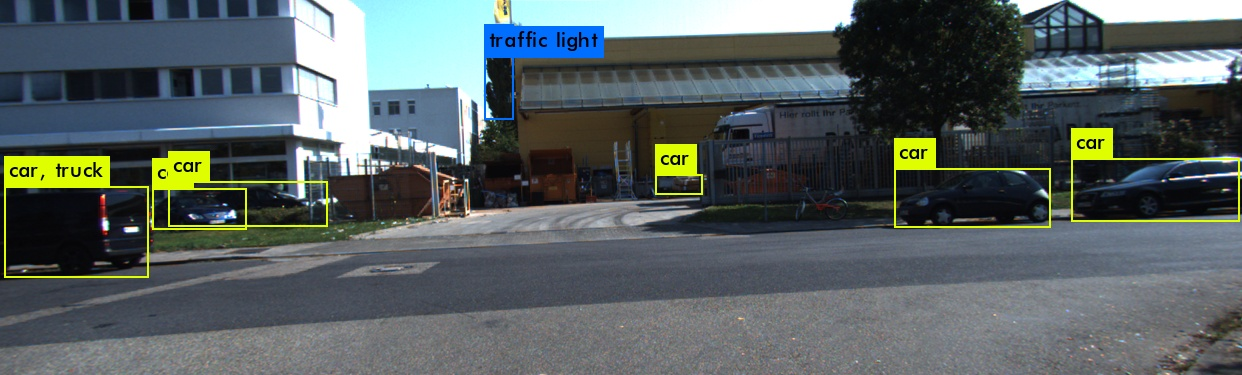
\includegraphics[width=\textwidth]{img/object-detection/kitti-4.jpg}
		\caption{Object detection on an urban area. Classification and bounding box dimensions and position are accurate, with exception to the traffic light bounding box, that is mistaken with a tree top and two cars in the middle of the image that are labelled as only one car.}
		\label{fig:kitti-yolo-3}
	\end{subfigure}
	\\ \vspace{4mm}
	\begin{subfigure}[c]{0.8\textwidth}
		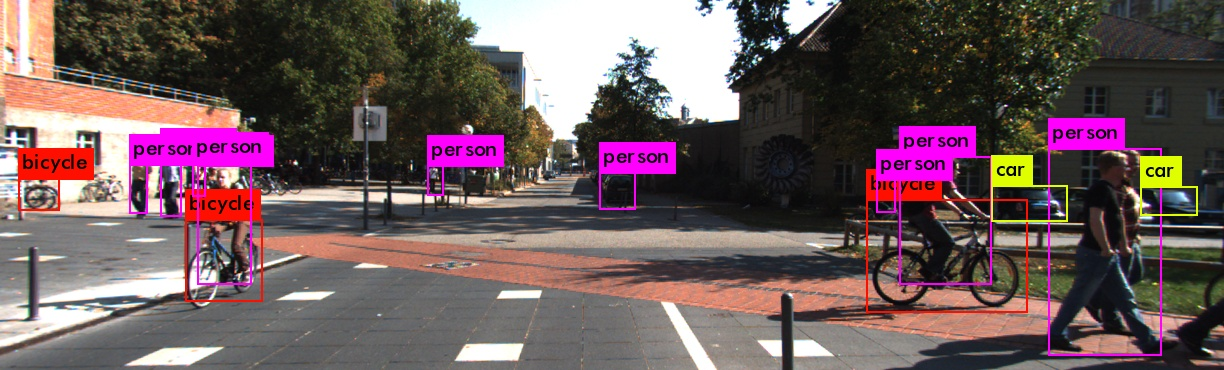
\includegraphics[width=\textwidth]{img/object-detection/kitti-2.jpg}
		\caption{Object detection on Karlsruhe Institute of Technology \textit{campus}. There are two detection errors on this image. In the center, two road poles and a car are labelled as a person. On the right, two persons are grouped together in one bounding box.}
		\label{fig:kitti-yolo-2}
	\end{subfigure}
	\caption{Object detection results for the \ac{kitti} dataset, using \ac{yolo}v3 with a confidence threshold of 30\%, trained for the \ac{coco}'s image dataset. With the specifications present on table~\ref{tab:computer-specs}, a 1.3 to 1.8 \ac{fps} were registered when classifying the images.}
	\label{fig:kitti-object-detection}
\end{figure}


\subsubsection{Experimental Data acquired}
Exemplary results of the object detection method applied to the experimental data gathered on a \ac{msl} robotic football field, at the \acf{irislab}, are presented on figure~\ref{fig:experimental-object-detection}. The confidence threshold of \ac{yolo} is set to 30\% and with the specifications present on table~\ref{tab:computer-specs}, a 1.1 to 1.4 \ac{fps} were registered when classifying the images.

Since experimental data was stored on raw format, as detailed on Section~\ref{sec:calibration:extrinsic}, de-Bayering and rectification of the raw image must be done, using the \texttt{image\_proc} package, before sending the data to the \texttt{Darknet} framework.

On the left sub-figure,~\ref{fig:experimental-yolo-2}, image object detection is done on ground-truth camera data. Objects on the background are detected, even if faraway from the camera ($\approx\SI{14}{\meter}$) and out of focus (see Sub-section~\ref{subsec:calibration:dof-and-calibration-object}). A human dummy is classified as a person and a knob is mistakenly labelled as a sports ball. The chair and the television monitor are correctly classified, but their bounding boxes dimension are smaller than they should be, because of partial occlusion.
On the right sub-figure,~\ref{fig:experimental-yolo-1}, calibrated data is used for image detection. Objects on the front are detected: a sports ball, a chair and a person. The last two ones are detected with good bounding box accuracy, even if occluded. On the background, no objects are detected, since the objects detected on sub-figure~\ref{fig:experimental-yolo-2} are occluded. 

\begin{figure}[!ht]
	\centering
	\begin{subfigure}[t]{0.45\textwidth}
		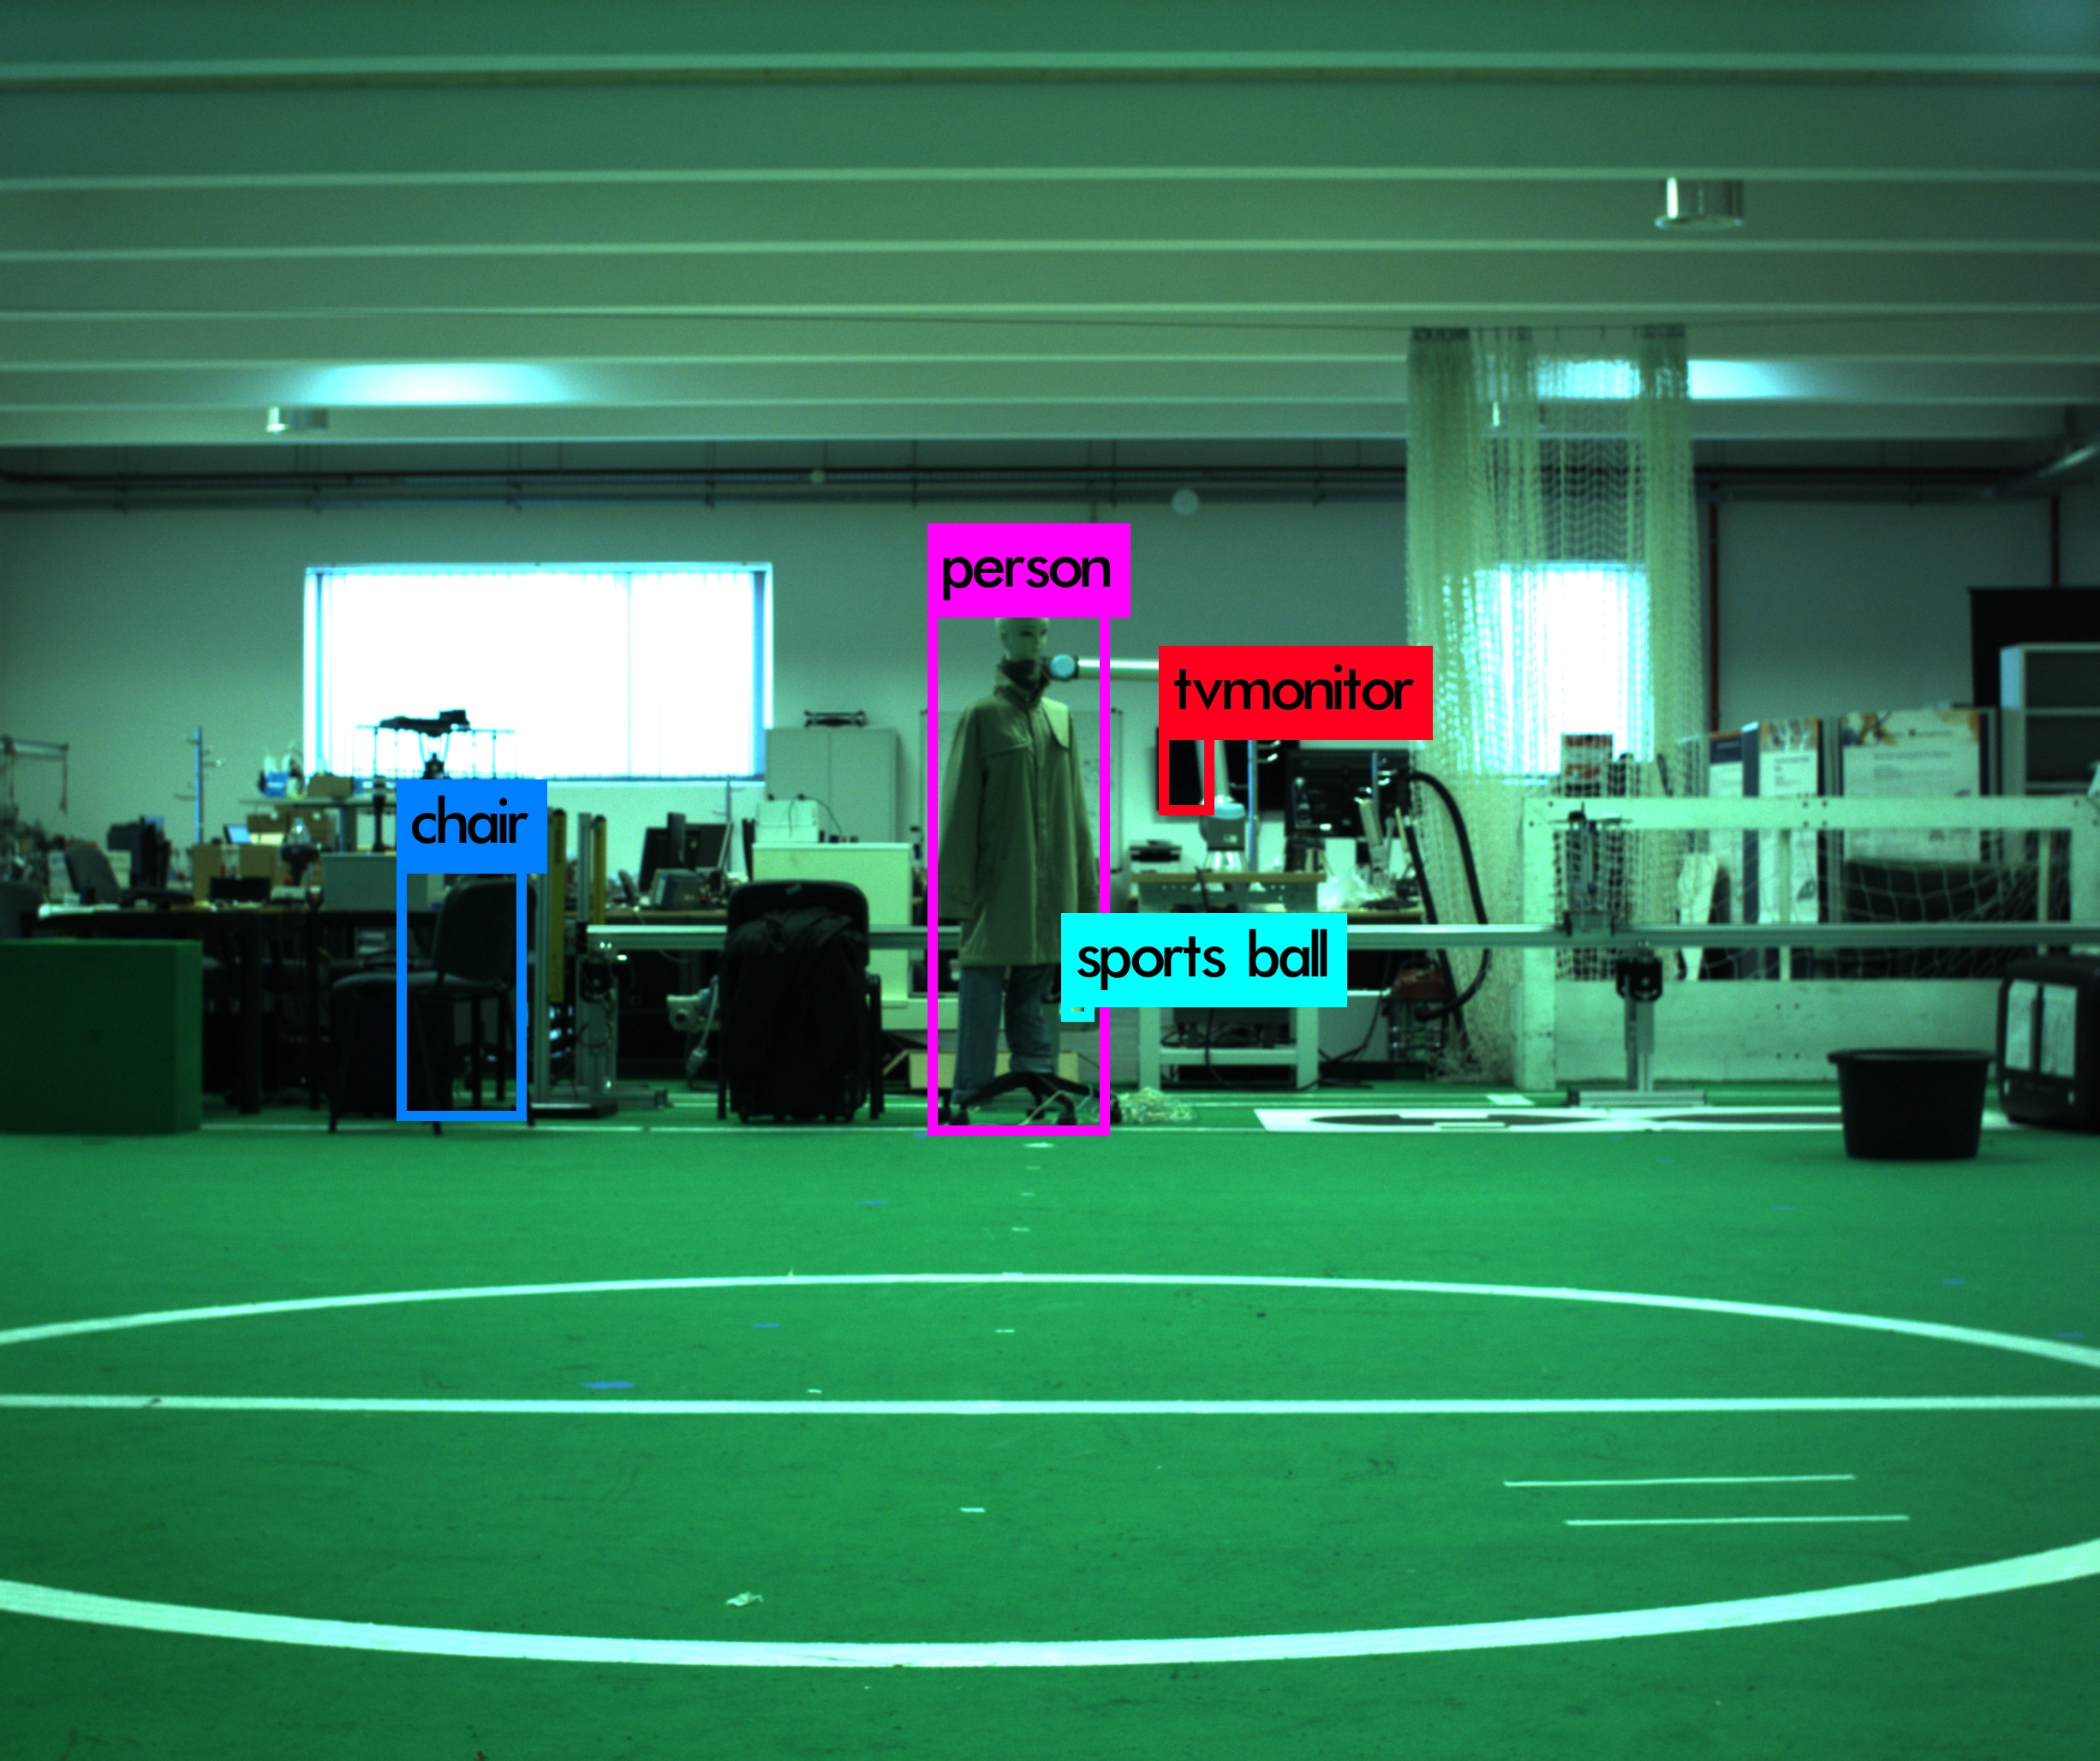
\includegraphics[width=\textwidth]{img/object-detection/experimental-2.jpg}
		\caption{}
		\label{fig:experimental-yolo-2}
	\end{subfigure}
	\qquad
	\begin{subfigure}[t]{0.45\textwidth}
		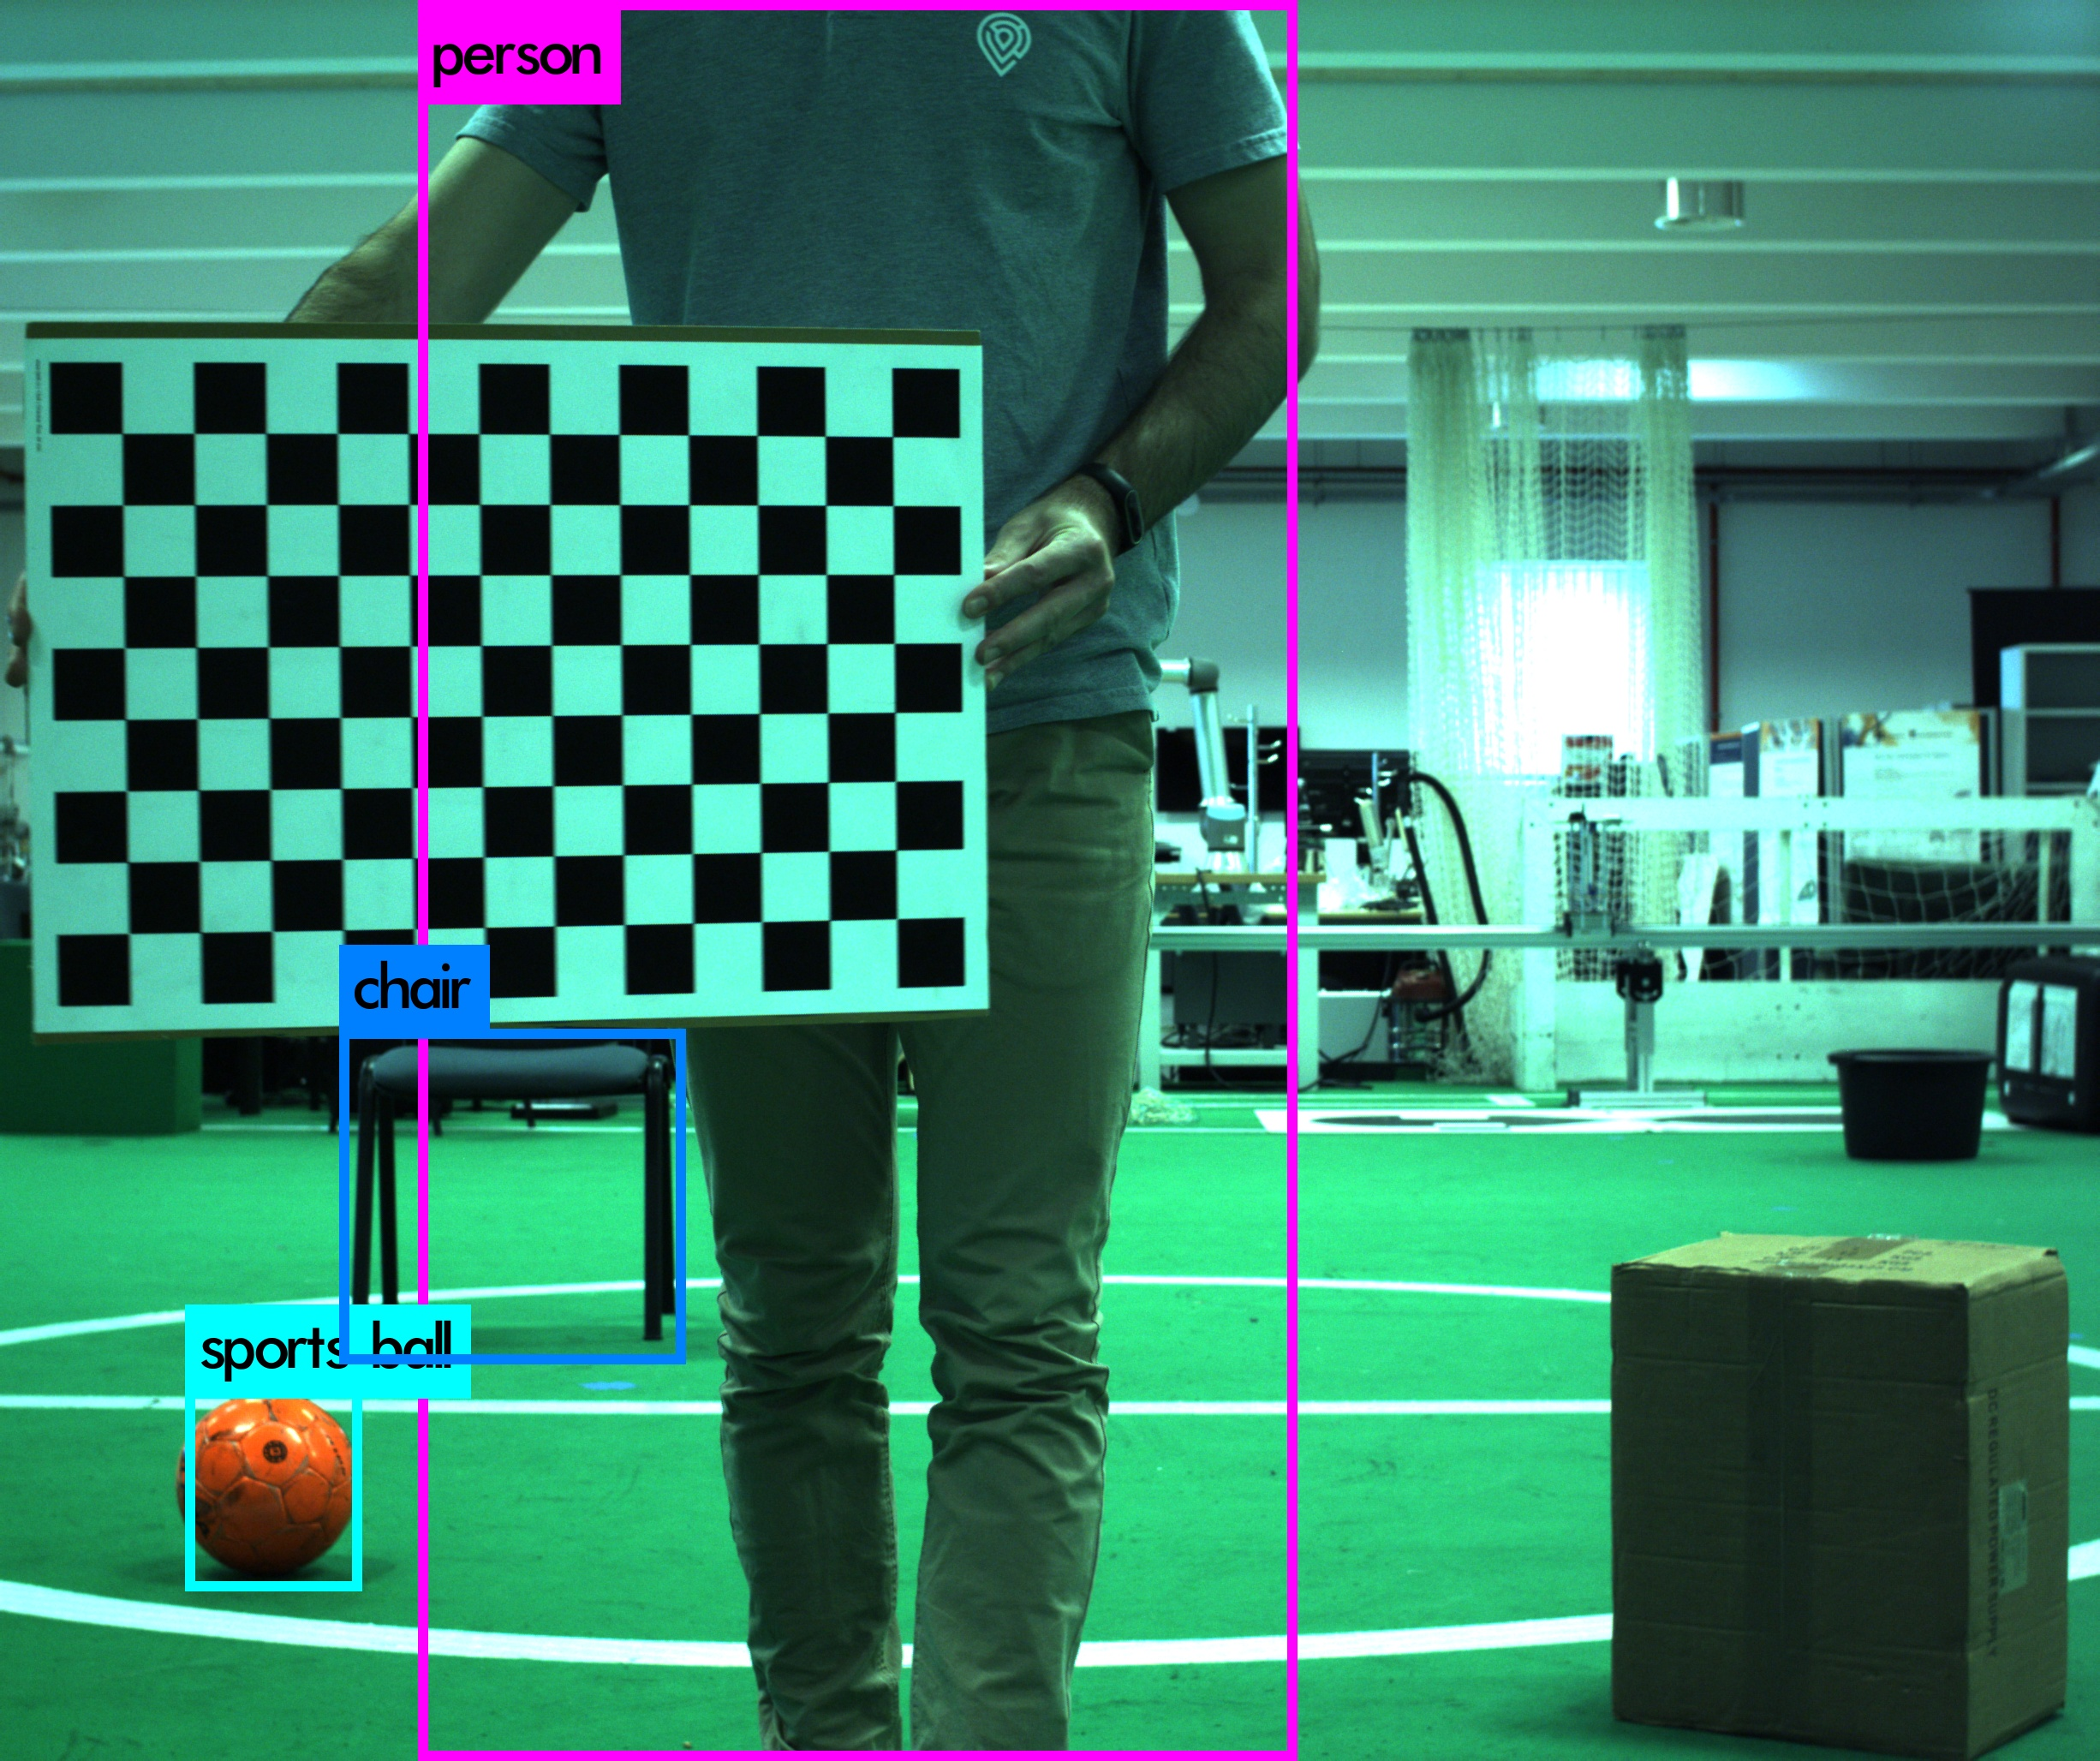
\includegraphics[width=\textwidth]{img/object-detection/experimental-1.jpg}
		\caption{}
		\label{fig:experimental-yolo-1}
	\end{subfigure}
	\caption{Object detection results for the experimental data gathered on a \ac{msl} robotic football field, at \ac{irislab}. \ac{yolo}v3 is used with a confidence threshold of 30\% and trained for the \ac{coco}'s image dataset. With the specifications present on table~\ref{tab:computer-specs}, a 1.1 to 1.4 \ac{fps} were registered when classifying the images. Note that since the data was stored on a raw format, de-Bayerization and rectification need to be performed by \texttt{image\_proc} \ac{ros} package before the RGB images are feed to the \texttt{Darknet}. In sub-figure~\ref{fig:experimental-yolo-2}, a human dummy is detected as a person and a knob is confused with a sports ball. On the back, the tv monitor is correctly classified, but the bounding box is smaller, since it is occluded by the robotic arm. In sub-figure~\ref{fig:experimental-yolo-1}, despite the occlusion of the chair and person, \ac{yolo} is capable of recognizing them both with accuracy.}
	\label{fig:experimental-object-detection}
\end{figure}


\section{Correspondences between objects in image and point-cloud}
An experimental setup with an intrinsically calibrated camera and \ac{lidar}, on which their rigid body transformation is known\footnote{The method used to determine this rigid body transformation on our experimental dataset is outlined on Section~\ref{sec:calibration:extrinsic}. Chapter~\ref{chapter:calibration} details all the calibration procedures that are pre-required for this section. For \ac{kitti} dataset, such transformations are already given.}, allows data conversion between its two coordinate frames, as shown previously in Chapter~\ref{chapter:sensor-fusion}. 

Matching the camera's \acp{roi} with \ac{lidar}'s require converting the data to a common coordinate frame between the two sensors and then using a matching algorithm to select the point cloud points that correspond to the classified object on the image.

Determining the point cloud's \ac{roi} from the image bounding boxes implies establishing a $2D \leftrightarrow 3D$ correspondence between the data, that is used to match \acp{roi} on the two sensors. Similar to the methods for fusing different sensory data on Chapter~\ref{chapter:sensor-fusion}, two solutions based on the same principle are possible:

\begin{enumerate}
	\item The 2D pixels are converted to a 3D ray, referenced on the \ac{lidar} coordinate frame. This method uses a technique of ray-casting, computing the rays from the camera sensor center that pass through the pixel coordinates;
	\item The 3D points registered by the \ac{lidar} are projected to the image pixels plane, ``converting a two-dimensional \ac{roi} to a tridimensional \ac{roi}, A tridimensional bounding box is estimated and drawn, for visualization purposes, on the point cloud. 
\end{enumerate}

In this section, the implementation of both methods is presented, along with their results and a brief comparison. This section explains the implementation for computing the point cloud bounding boxes, by using the information of the image bounding boxes obtained with \ac{yolo}, as detailed on Section~\ref{sec:object-detection:image}. The results for every stage of the processing chain are also given.


\subsection{\texttt{Darknet-ros} Package Limitations and Contributions}
\label{subsec:object-detection:darknet-contribution}
\texttt{Darknet-ros} encapsulates the \texttt{Darknet} framework and allows its connection with other nodes on a \ac{ros} network. Excluding its interface for \ac{nn} configuration (\ac{nn} model and weights) and data input topics, that are detailed on~\cite{MarkoBjelonic}, \texttt{darknet-ros} provides 3 output topics:

\begin{enumerate}
	\item \texttt{found\_object}: a standard integer message that indicates the number of objects found by the \texttt{Darknet} framework when running the desired \ac{nn} model;
	\item \texttt{detection\_image}: A \ac{ros} image topic, similar to its input image topic, but with the detection bounding boxes drawn;
	\item \texttt{bboxes}: a custom message topic that contains a header with metadata and an array of bounding boxes detected on the image. Each bounding box element of this array indicates its class, ID, probability and the minimum and maximum points that define the image bounding box for that object;
\end{enumerate}

For this work, precise synchronization between the point cloud and \texttt{darknet}'s outputs is required. However, \texttt{darknet-ros}' does not provide an interface with such functionality, lacking information to synchronise the \texttt{found\_objects} topic with other topics.

To mitigate this problem, we propose an improvement on \texttt{darknet-ros} package. Our proposal consists on defining a custom message for \texttt{found\_objects} topic that additionally to the standard integer indicating the found objects' number, also contains a header with the time stamps and frame id for synchronization. The \texttt{darknet-ros} core code was also changed to publish this new message type under \texttt{found\_objects} topic, ensuring also backwards compatibility.

Those changes were later submitted to the original author of \texttt{darknet-ros}, which were accepted and merged with the publicly available source code~\cite{MarkoBjelonic}.


\subsection{Ray Casting}
\label{subsec:object-detection:ray-casting}
The first implemented algorithm to match image and point cloud \acp{roi} involves a technique of ray casting, i.e., casting a ray from the camera center that passes thought the desired pixel, projecting it from the two-dimensional image representation to a three-dimensional, that is suited for comparison with \ac{lidar} data.

After data conversion from one coordinate frame to the other, using the rigid body transformation determined on Section~\ref{sec:calibration:extrinsic}, ray-casting allows the determination of 4 lines that delimit a 3D section of the point cloud, by casting the corners of the image bounding box. These 4 lines, transformed to the \ac{lidar} coordinate frame, define the boundaries of an infinite rectangular pyramid, with its vertex on the \ac{lidar} center. Considering a near and far parallel cut planes that are perpendicular to the pyramid orientation, a pyramidal frustum is obtained (see figure~\ref{fig:pyramid-frustum}), containing all the point cloud points that are part of the tridimensional \ac{roi} for the object detected.  

\begin{figure}[H]
	\centering
	\def\svgwidth{0.3\columnwidth}
	\graphicspath{{img/image-object-to-point-cloud/}}
	\includesvg{img/image-object-to-point-cloud/pyramid-frustum}
	\caption{Pyramid Frustum. The gray section corresponds to the pyramid frustum volume between the near and far plane on the boundaries defined by the pyramid.}
	\label{fig:pyramid-frustum}
\end{figure}

Performing a frustum segmentation on the point cloud requires four steps:

\begin{itemize}
	\item Back-project the pixels to rays, defining the boundaries of the point cloud;
	\item Compute the pure rotation coefficients that align the \ac{lidar} coordinate frame to the coordinate frame oriented to the \ac{roi};
	\item Calculate the vertical and horizontal \acf{fov} of the pyramid frustum;
	\item Determine the limits of the near and far cut planes.
\end{itemize}

\subsubsection{Back-project the pixels to rays}
Projecting pixels to a ray (also called back projection) is the inverse process that is used to create an image on a camera\footnote{A camera projects the world points to a two-dimensional plane. See Sub-section~\ref{subsec:sota:camera-geometry}}. The projection matrix defined in equation~\eqref{eq:camera_transform_full}, if inverted, may be used to calculate the transformation matrix that  back projects pixels into rays.

Since on our implementation, the transformation between different coordinate frames is done separately from the back-projection algorithm, the image pixels are already defined on the camera's coordinate frame. Therefore, the joint rotation and translation matrix, $\begin{bmatrix} R|t \end{bmatrix}$, is equal to the identity and a zero column vector, respectively, and does not need to be accounted for.

Following Hartley's and Zisserman's book~\cite{mvg_book}, our back-projection operation degenerates to computing the inverse of the intrinsic camera matrix, $K$, and multiply that inverse by the pixel coordinates referenced in affine coordinates, detailed in equation~\eqref{eq:back-projection}. The rotation and translation to convert the rays from the camera's coordinate frame to \ac{lidar}'s are applied after the ray-casting operation.

\begin{align}
	\label{eq:back-projection}
	\begin{bmatrix}
		X \\
		Y \\
		Z
	\end{bmatrix}
	 & = K^{-1} 
	\begin{bmatrix}
		u \\
		v \\
		1
	\end{bmatrix}
\qquad , \quad
	K = 
	\begin{bmatrix}
		f_x & 0 & c_x \\
		0 & f_y & c_y \\
		0 & 0 & 1.0
	\end{bmatrix}
\nonumber \\	 
	&  = 
	\begin{bmatrix}
	\frac{1}{f_x} & 0 & -\frac{c_x}{f_x} \\
	0 & \frac{1}{f_y}  & -\frac{c_y}{f_y} \\
	0 & 0 & 1.0 
	\end{bmatrix}
	\begin{bmatrix}
		u \\
		v \\
		1
	\end{bmatrix}
\end{align}

\subsubsection{Rotation from the \ac{lidar} coordinate frames to the bounding boxes' coordinate frame}
The rotation of the \ac{lidar} coordinate frame to each of the bounding boxes coordinate frames is obtained by calculating the angle between the two rays: the ray from the camera center to the image bounding box center and the ray from the camera center to the image center. 

Let $B^\text{center}$ be the image bounding box center, which can be calculated using equation~\eqref{eq:bboxes-pixel-center} and $C^\text{center}$ be the image center, that corresponds to the intrinsic camera parameters $c_i, \forall i \in \{x, y\}$, as denoted in equation~\eqref{eq:image-pixel-center}.

\begin{equation}
	\label{eq:bboxes-pixel-center}	
B^\text{center} = \left(\frac{x^{\text{bounding box}}_{min} + x^{\text{bounding box}}_{max}}{2}, \frac{y^{\text{bounding box}}_{min} + y^{\text{bounding box}}_{max}}{2},\right)
\end{equation}

\begin{equation}
\label{eq:image-pixel-center}
C^\text{center} = (c_x, c_y)
\end{equation}

%Considering that the representation of a generic point $P = (x, y, z)$ in affine coordinates is given by $P_\text{affine} = \left[P | 1\right]^T$, where $T$ represents the matrix transpose, and consider that in this case, $P \in \{B^\text{center}, C^\text{center} \}$. 
Denote  the ray projected by the camera origin that passes through the pixels defined by the points $B^\text{center}_\text{affine}$ and $C^\text{center}_\text{affine}$, as $\vec{b}$ and $\vec{c}$, respectively, where $\vec{b}$ and $\vec{c}$ are determined using equation~\eqref{eq:back-projection}, that $\vec{b} = K^{-1} \times B^\text{center}_\text{affine}$ and $\vec{c} = K^{-1} \times C^\text{center}_\text{affine}$.

By applying the rigid body transformation between the camera and the \ac{lidar} determined in Section~\ref{sec:calibration:extrinsic}, let us define vector $\vec{b'}$ and $\vec{c'}$ as the vectors $\vec{b}$ and $\vec{c}$, referenced on the \ac{lidar} coordinate frame, respectively.

Then, the rotation of the \ac{lidar} coordinate frame to a new frame oriented to the bounding box can then be obtained by calculating the quaternion that defines the angle of rotation between vector $\vec{c'}$ and $\vec{b'}$~\cite{mvg_book}. The rotation transformation can be denoted as $\mathbf{q}_{c'b'}$, which is capable of projecting a line from the coordinate frame of the bounding box, $b'$, to the \ac{lidar} coordinate frame, $c'$. Afterwards, the quaternion can be converted to a rotation matrix~\cite{Dai2015, mvg_book}, so that the rotation can be applied together with order rotations already obtained.

\subsubsection{Horizontal and Vertical \ac{fov} of the pyramidal frustum}
The horizontal and vertical \ac{fov} are determined on the image plan. First, the angle between the image center and each of the bounding box limits (upper and lower) are calculated for the two dimensions, $x$ and $y$. Then, the difference between the upper and lower angles is computed to obtain the \ac{fov} on that axis.

Let $\theta^\text{upper limit}_i$ denote the upper limit of the image bounding box, on the generic $i$ axis, that can be replaced by $x$ or $y$, and $\theta^\text{lower limit}_i$ represent the lower limit of that same axis. Consider the image axis origin to be at the center of the image and the \ac{fov} of the bounding box can be defined by $\Theta^\text{FOV}_i$ on equation~\eqref{eq:image-fov}, for that same generic axis $i$.

\begin{equation}
	\label{eq:image-fov}
	\Theta^{FOV}_i = \theta^\text{upper limit}_i - \theta^\text{lower limit}_i, \qquad \forall i \in \{x, y\}
\end{equation}

With some trigonometry and camera geometry\footnote{Camera geometry is detailed on subsection~\ref{subsec:sota:camera-geometry}. Figure~\ref{fig:pinhole_camera_model} might be interesting revisiting before continuing.} one can see that:

\begin{align}
	\theta^\text{upper limit}_i = \tan\left(\frac{\max(i)}{f_i}\right), \qquad i \in \{x, y\} \\
	\theta^\text{lower limit}_i = \tan\left(\frac{\min(i)}{f_i}\right), \qquad i \in \{x, y\} 
\end{align}

\subsubsection{Determine the near and far cut planes limits}
The Near and Far Cut Planes may be defined by the data and \ac{lidar} constraints. Following the datasheet of the VLP-16~\cite{vlp16}, the \ac{lidar} used on the experimental setup, and HDL-64~\cite{VelodyneHDL64}, the \ac{lidar} used on the \ac{kitti} dataset, the Near Cut Plane is defined as \SI{1}{\meter}, since the \acp{lidar} cannot detect smaller distances.

Due to point cloud data scarcity, both on the experimental and  \ac{kitti} dataset, a Far Plane of \SI{30}{\meter} is enough to guarantee that all the objects of interest on the \ac{fov} are present.

\subsubsection{Implementation}
Using the constrains and methods detailed before, a \ac{ros} node, \texttt{image\_bbox\_to\_point\_cloud\_node}, is written to perform frustum filtering on the point cloud using the image bounding boxes determined by \texttt{darknet-ros}. The node diagram is shown on figure~\ref{fig:ros-graph-frustum}, where the node \texttt{Kitti\_dataset} is a \texttt{rosbag} player and \texttt{darknet-ros} is the node described in Section~\ref{sec:object-detection:image}, responsible for image object detection. \texttt{Rviz} is the \ac{ros} visualizer, configured to show the transformations between the coordinate frames, the original point cloud and the frustum filtered point cloud.

\begin{figure}[t]
	\centering
	\def\svgwidth{\columnwidth}
	\graphicspath{{img/image-object-to-point-cloud/}}
	\includesvg{img/image-object-to-point-cloud/frustum}
	\caption{\ac{ros} node graph corresponding to the implementation of the Point Cloud Frustum Filter node from the image bounding boxes.}
	\label{fig:ros-graph-frustum}
\end{figure}


This node is implemented using \ac{pcl} frustum filter algorithm and Eigen library. Eigen is a C++ library for linear algebra, matrix and vector operations and geometric transformations, among other features~\cite{Eigenv3}. The pose of each of the bounding boxes is also computed, either towards the \ac{lidar}'s and the \ac{pcl}'s frustum algorithm coordinate frame. 

Several alternatives to the methods described above (for \ac{fov} calculation, determine the \ac{lidar} rotation, for example) have been implemented, but are not going to be described here. Several auxiliary functions (for debugging, visualization and computing other features) will also not be addressed, since they require a more in depth explanation of the implementation, that was no interest for such document. 


\subsubsection{Results}
Applying the frustum filtering methodology described on the sub-sections above to the point cloud data can be seen on figure~\ref{fig:bbox-correspondences-on-kitti}. The dark grey points correspond to the original point cloud, \texttt{velodyne\_points}, and the orange points to the frustum filtered point cloud, \texttt{frustum\_filtered\_point\_cloud}.

The red arrows represent the pose of each of the objects \acp{roi} and the yellow arrows the pose of those objects on the frustum filter coordinate frame, which differs from the Velodyne \ac{lidar} coordinate frame. Although the Velodyne \ac{lidar} coordinate frame is z upwards, y leftwards and z forward\footnote{Velodyne \ac{lidar} coordinate frame on \ac{kitti} dataset can be seen better in figure~\ref{fig:kitti-tf-frames} on Sub-section~\ref{subsec:calibration:kitti-comparison} or on \ac{kitti}'s paper~\cite{Geiger2013a}.}; the \ac{pcl} frustum filter coordinate frame is y upwards, z rightwards and x forward.

\begin{figure}[ht]
	\centering
	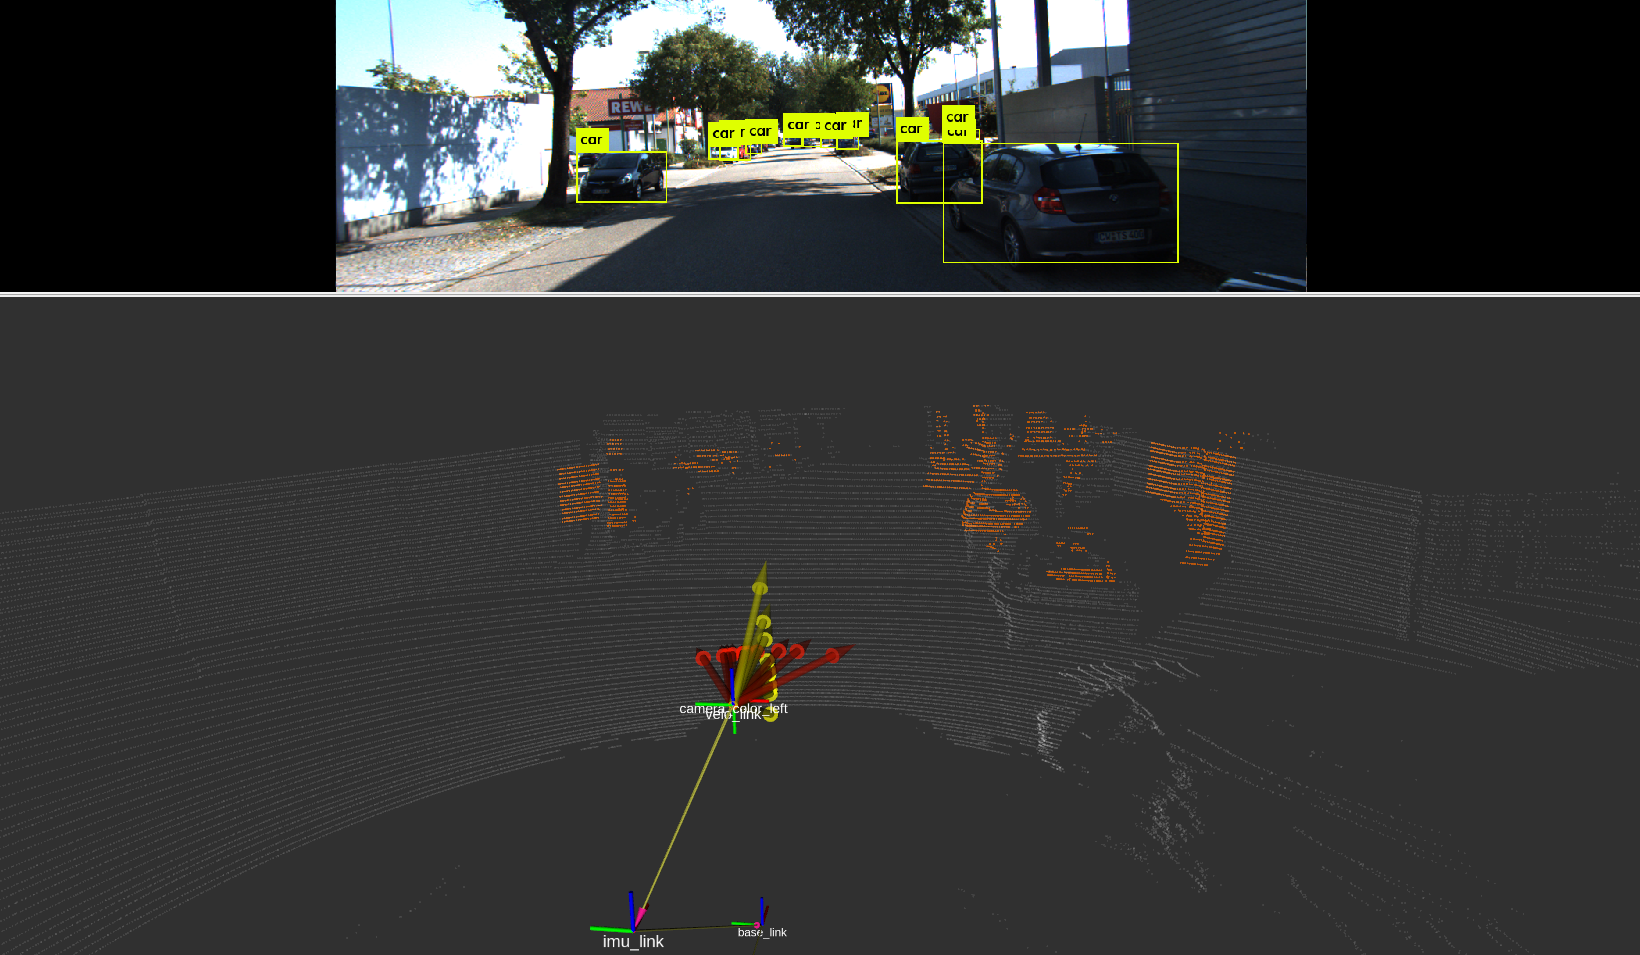
\includegraphics[width=0.8\textwidth]{img/image-object-to-point-cloud/bbox_correspondences_on_kitti.png}
	\caption{Pyramidal Frustum filtering of \acp{roi} given by the image bounding boxes on \ac{lidar} data. The dark grey points correspond to the unfiltered \ac{lidar} point cloud and the orange points to the ones selected by frustum filtering. One can see that there is a discrepancy between the objects of interest on the point cloud (cars) and the selected \acp{roi} by the algorithm. The red arrows point to each of the \acp{roi} on the \ac{lidar} coordinate frame and the yellow arrows point to the \acp {roi} on the \ac{pcl}'s frustum filter algorithm coordinate frame.}
	\label{fig:bbox-correspondences-on-kitti}
\end{figure}

The results shown on figure~\ref{fig:bbox-correspondences-on-kitti} are not as anticipated. Mismatches between the bounding boxes on the image and \acp{roi} selected by the frustum filter are not coincident. Analyzing the unfiltered (gray points) and the filtered point cloud (orange points), one can notice that some regions of the dark grey point cloud that correspond to the cars (that are detected on the image), are not considered a \ac{roi} and therefore are not filtered by the algorithms implemented and are not part of the filtered point cloud. Also, in contrast, some regions that have not been considered as \acp{roi} on the image are selected on the point cloud.

A mismatch on determining the correspondences between the \acp{roi} on the image and \ac{lidar} has been made, that can either be from the coordinate frames conversion, calculation of the \ac{lidar} rotation and \ac{fov} determination or by a combination of errors/imprecisions made in one of these steps. The implementation requires some third party libraries, such as \ac{pcl}, \ac{opencv} and Eigen, to be integrated in order to filter the point cloud, which might also be the source of the problems.

The implementation was thoroughly debugged but the cause of the mismatch was not found. Therefore, a simpler algorithm to match the \acp{roi} between camera and \ac{lidar} was developed, to fulfill the thesis objective of computing correspondences between image and point cloud objects.


\subsection{Projecting \ac{lidar} points to the image}
\label{subsec:object-detection:projection-correspondences}

The alternative method to establish correspondences is similar to the one used for Sensor Fusion, detailed in Chapter~\ref{chapter:sensor-fusion}. The difference between the implementation on the latter chapter and this is that instead of comparing if the projected \ac{lidar} points correspond to a pixel in the image, they must also be contained in an image bounding box. 

This approach has a few drawbacks when compared with the previously described in sub-Section~\ref{subsec:object-detection:ray-casting}, but is easier and less complex. It requires only four steps, some already implemented previously:

\begin{enumerate}
	\item Transform the \ac{lidar} point cloud from the \ac{lidar} coordinate frame to the camera's coordinate frame, as detailed in sub-Section~\ref{subsec:calibration:calibration-method}. Similar to the conversion in Chapter~\ref{chapter:sensor-fusion}, the coordinate conversion frame is the rigid body transformation determined in section~\ref{sec:calibration:extrinsic}.;
	\item Project the \ac{lidar} point cloud points to the camera's image two-dimensional planes, using the methodology detailed in sub-section~\ref{subsec:sensor-fusion-lidar-to-camera};
	\item Check if the projected point cloud points correspond to image pixels inside of image bounding boxes. If true, save the index of the point cloud point;
	\item Using \ac{pcl}'s Extract Indices filter, a new point cloud is created from the original, containing the indexes selected on the previous step.
\end{enumerate}

However, using this method, every point of the point cloud is treated independently of the others. Since the point cloud is not organised, causing the spatial relation of the \acp{roi} on point cloud to not be preserved, the information of the detected objects on image (class, probability) obtained through the image object detection of Section~\ref{sec:object-detection:image} is harder to transfer to the corresponding points on the point cloud.


\subsubsection{Implementation}
The methodology chosen builds upon the implementation detailed on section~\ref{sec:object-detection:image}. A new node, \texttt{correspondences\_finder}, responsible for extracting the indices and  publishing a filtered point cloud, is implemented. The \texttt{filtered\_point\_cloud} contains all the points that belong to the \acp{roi} correspondent to the image bounding boxes. 

The node is agnostic about the objects that are identified by the image object detection algorithms, considering only the bounding box dimensions and ignoring its class and confidence. Considering the mathematical notation of a bounding box as $bbox^i_j$, where $i$ corresponds to the bounding box index on \texttt{darknet-ros}' \texttt{bboxes} message and $j$ the coordinate of the bounding box, such as $j \in \{x, y\}$. Let also the number of the bounding boxes index be denoted as $\text{found\_object}$. A correspondence is made when the point cloud projection coordinates are such that a given point cloud point $P = (p_x, p_y,p_z)$ verifies equation~\eqref{eq:correspondences-condition}.

\begin{align}
	\label{eq:correspondences-condition}
	\forall i \in & [0, \ldots, \text{found\_object}], \nonumber \\ 
			& \exists P \in [\min(bbox^i_x), \max(bbox^i_x)] \cap [\min(bbox^i_y), \max(bbox^i_y)] 
\end{align}

The node diagram is presented on figure~\ref{fig:correspondences-finder-standalone}. Similar to image~\ref{fig:bbox-correspondences-on-kitti}, the implementation requires the usage of \texttt{Darknet-ros} to compute the image bounding boxes. The two alternatives are completely interchangeable, publishing the same type of message (a point cloud) and receiving the same inputs: the original \ac{lidar} point cloud, coordinate frame transforms and \texttt{darknet-ros} bounding boxes message and the number of detected objects.

\begin{figure}[!ht]
	\centering
	\def\svgwidth{\columnwidth}
	\graphicspath{{img/image-object-to-point-cloud/}}
	\includesvg{img/image-object-to-point-cloud/correspondences-finder-standalone}	
	\caption{\ac{ros} node diagram for \texttt{correspondences\_finder} implementation. It uses \texttt{Darknet-ros} to compute the image bounding boxes and a \texttt{rosbag} player to publish \ac{kitti} dataset data. The node publishes a point cloud message, \texttt{filtered\_point\_cloud}, containing the \ac{lidar} \acp{roi}' points, selected from the input point cloud, \texttt{velodyne\_points}.}
	\label{fig:correspondences-finder-standalone}
\end{figure}

\subsubsection{Results}
On figure~\ref{fig:projected-correspondences}, the results caused by applying the \texttt{correspondences\_finder} node are presented in lilac. The top part of the image presents the camera feed and the bottom the point cloud, with the relevant TF coordinate frames also visible. The  dark gray points represent the original \ac{lidar} data. 

Analyzing the results, we conclude that the objects of interest (on figure~\ref{fig:projected-correspondences}, cars) are filtered and part of the point cloud that contains the \acp{roi}, marked in lilac. In every \ac{roi}, however, some outlier points are also selected. This is because the image bounding boxes being rectangular, which results on non-optimal bounding boxes dimensions, causing the appearance of outliers when correspondences between the \ac{lidar} and camera data are made.

These outliers correspond to objects nearby of the detected object or to objects that occlude it. Normally, it contains a part of the background and the floor. Such outliers pose a problem, since points that do not belong to the object are being selected as part of it, and must be solved before any bounding box estimation can take place. Nevertheless, we consider the correspondences' detection to be correct and the results satisfactory.


\begin{figure}[!ht]
	\centering
	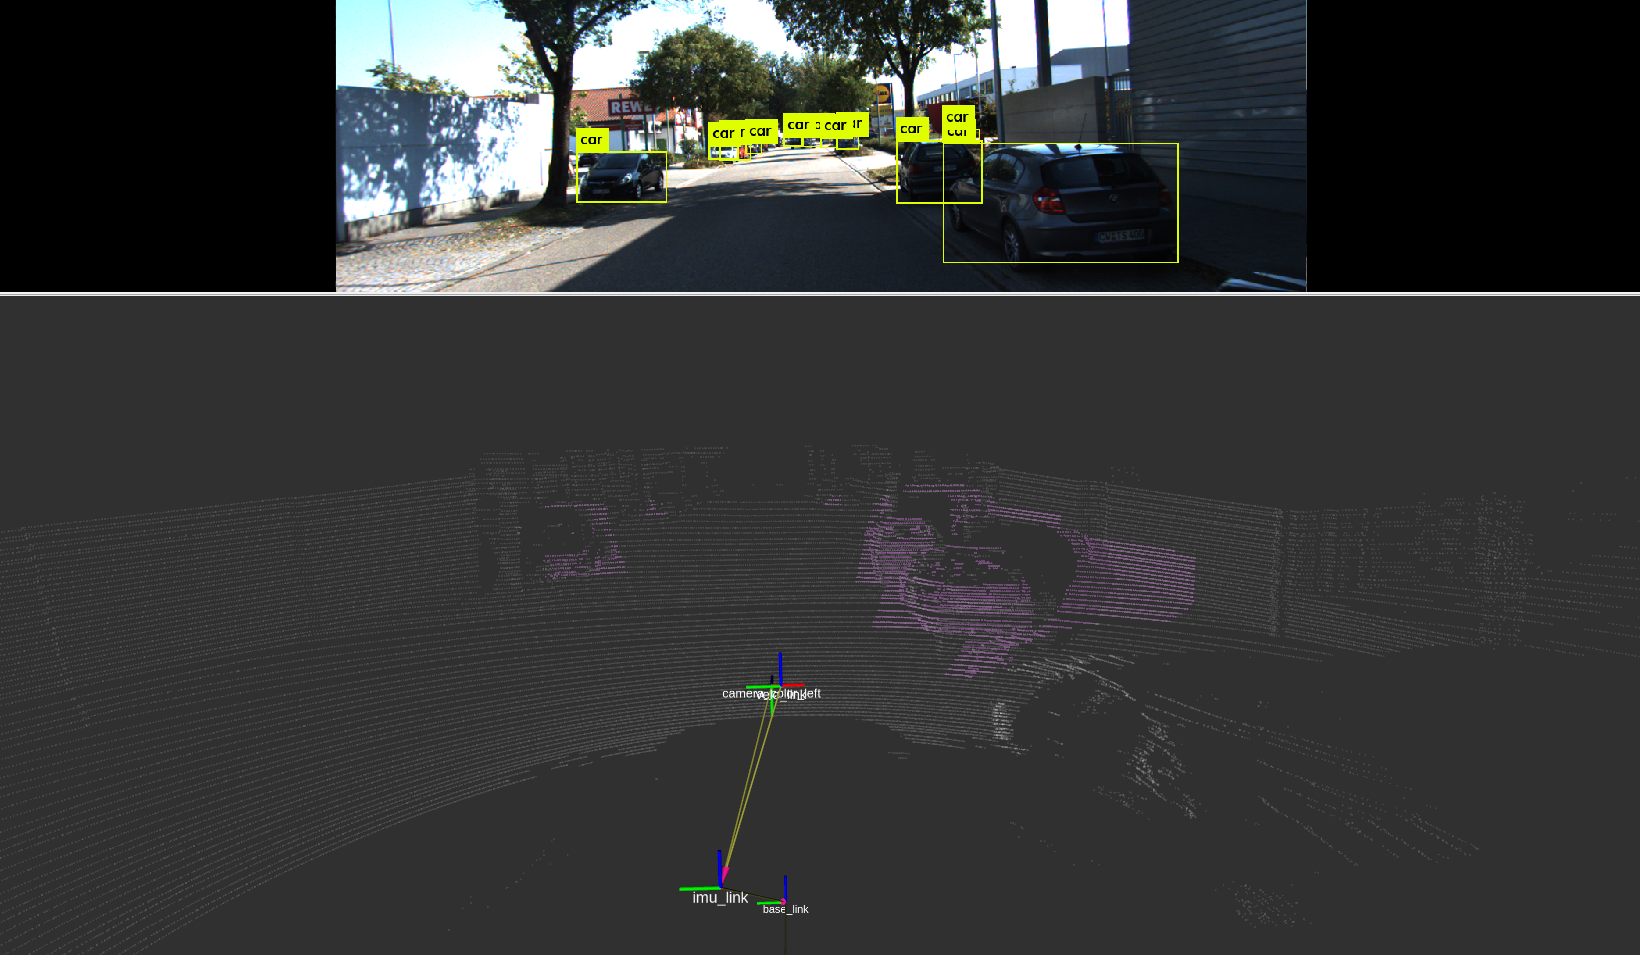
\includegraphics[width=0.8\textwidth]{img/image-object-to-point-cloud/projected_correspondences.png}
	\caption{Correspondences between the image bounding boxes and point cloud \acp{roi}. The dark grey points correspond to the unfiltered \ac{lidar} point cloud and the lilac points to the ones selected by the \texttt{correspondences\_finder} node, using the projection algorithm detailed. One can see that the cars that are detected on the image are filtered and marked by the algorithm. On those regions, some outliers are also present due to the bounding boxes being non-optimal to enclose the object dimensions.}
	\label{fig:projected-correspondences}
\end{figure}

\subsection{Comparison between the two methods}
The results of the two approaches can be compared on figure~\ref{fig:rois-matching-comparison}. In orange, the results of Sub-section~\ref{subsec:object-detection:ray-casting}, based on ray-casting and data conversion from the camera to \ac{lidar}; and in lilac, the results of Sub-section~\ref{subsec:object-detection:projection-correspondences}, based on projecting the \ac{lidar} points to the image plan and verifying which points laid inside the image bounding boxes limits.


\begin{figure}[!ht]
	\centering
	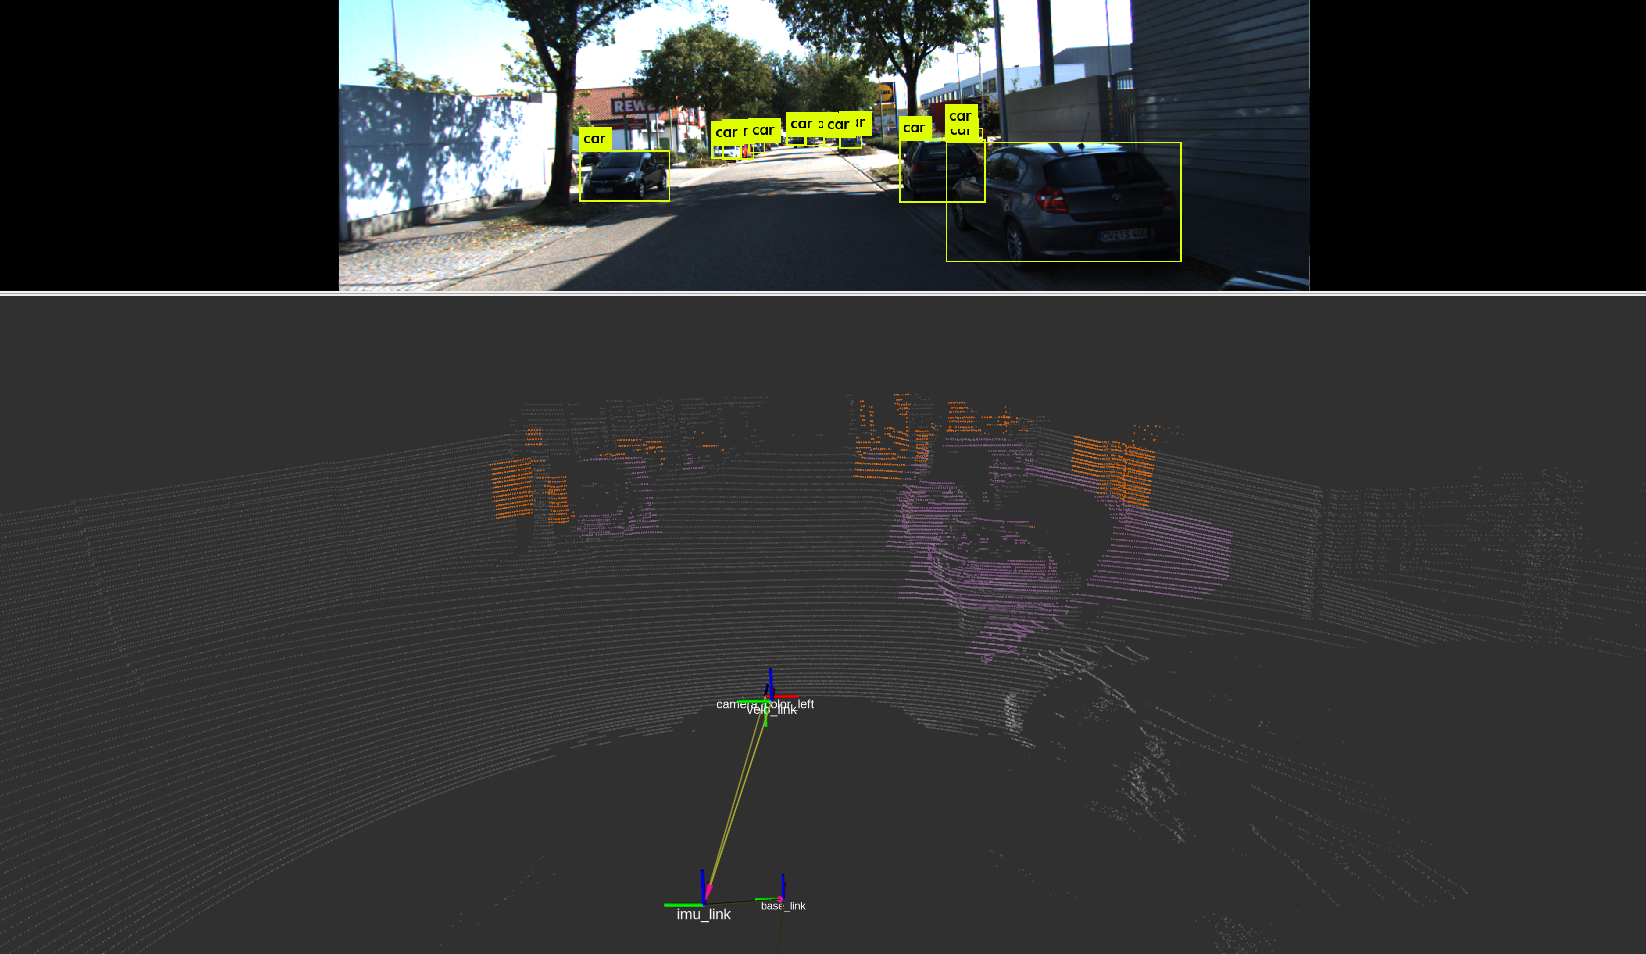
\includegraphics[width=0.8\textwidth]{img/image-object-to-point-cloud/rois-comparison.png}
	\caption{Comparison between the point cloud's \acp{roi} selected with the two algorithms: in lilac, using the \texttt{image\_bbox\_to\_point\_cloud\_node} (detailed in Sub-section~\ref{subsec:object-detection:ray-casting}); and in orange, using the \texttt{correspondences\_finder\_node} (detailed in Sub-Section~\ref{subsec:object-detection:projection-correspondences}). On the bottom of the image, a dark gray point cloud is also presented, showing the original point cloud gathered by the \ac{lidar}. Comparing with the top part of the image, which shows the camera feed, the lilac subset of the original point cloud identifies with better accuracy the point cloud \acp{roi} that correspond to the detected objects on the image.}
	\label{fig:rois-matching-comparison}
\end{figure}

After analyzing the comparison between both algorithms on figure~\ref{fig:rois-matching-comparison}, the solution chosen for detecting \acp{roi} on the point cloud using the image \acp{roi} represented as bounding boxes, is the one detailed in Sub-section~\ref{subsec:object-detection:projection-correspondences}, since the results are more accurate.

\subsection{3D Bounding Boxes and \aclp{roi}}
\label{subsec:object-detection:bounding-boxes-and-roi}
Estimating a \ac{roi} on a point cloud from an image has the caveat of requiring the conversion between a 2D object (a rectangle representing a bounding box on the image) to a 3D object (a parallelepiped representing a bounding box on the point cloud). As detailed in the Chapter~\ref{chapter:sensor-fusion}, such conversion requires the estimation of one degree of freedom, depth, whose information is absent from the image.

As detailed in this chapter, we want to draw a bounding box on the point cloud using only the information of the camera. Therefore, we need to estimate the depth of the 3D bounding box that contains all the points of an object that correspond to the object of interest on the image, that was classified during the image detection procedure (see Section~\ref{sec:object-detection:image}).

To reduce mismatches and improved the accuracy of the bounding boxes, before computing them, the point cloud is filtered using a voxel filter to uniform point cloud density on the already filtered \acp{roi}. The voxelized point cloud is then feed to a clustering algorithm, to select on the points of each \ac{roi} that correspond to the actual object of interest, reducing outliers. The resulting clusters are then used as input for the bounding box estimation algorithm.


\subsubsection{Voxelization}
To reduce the number of points on the filtered point cloud (speeding up the process) and to uniform point density, \ac{pcl}'s Voxel Grid filter is used to voxelize the point cloud. \ac{pcl}'s voxel grid creates a tridimensional grid of voxels that encapsulate all the point cloud points and, for every voxel, the centroid of the points within each voxel is computed, replacing all the voxel's points with its centroid.

On our experimental datasets, a voxel grid of \SI{0.04}{\centi\meter} was used, causing a reduction of 5\% to 15\% on the filtered point cloud number of points.

\subsubsection{Clustering}
As seen in figure~\ref{fig:projected-correspondences}, the filtered \acp{roi} contain outliers that do not belong to the object of interest detected on the image. Those outliers originate from the non-optimal image bounding box dimensions, and must be removed (or at least reduced) to ensure a good tridimensional bounding box fitting.

Since the point cloud density varies with distance, clustering will cause the distant \acp{roi} to be removed and the closer \acp{roi}, since a voxel filter has been applied, to be filtered, since the point cloud density is approximately uniform for a single object. Our implementation uses \ac{pcl}'s Euclidean Clustering algorithm, with a search method based on K-Dimensional tree\footnote{On our case, K$=3$, since the point cloud data only contains 3 euclidean coordinates: x, y, z.} for space partitioning and point cloud organization.

The Euclidean Filter uses 3 parameters:

\begin{enumerate}
	\item \textbf{Cluster tolerance:} Maximum distance between the points of the cluster, measuring using a Euclidean L2 norm. If the L2 norm between a cluster point and a candidate cluster point is greater than this parameter, the candidate point is not part of the cluster;
	\item \textbf{Minimum cluster size:} Minimum number of points, that verify the cluster tolerance condition, that are required to create a cluster. If the number of points that verify condition 1 are smaller than this number, a cluster is not created;
	\item \textbf{Maximum cluster size:} Maximum number of points, that verify the cluster tolerance condition, that can be part of a cluster. The number of points that verify condition 1 must be smaller or equal than this parameter, otherwise a cluster is not created.
\end{enumerate}

To ease the estimation of the filter parameters, \texttt{correspondences\_finder\_node} was changed to contain a \ac{ros} dynamic reconfigure server, allowing the modification of the filter parameters in real-time during program execution. 

To tune the parameters, minimum and maximum cluster size were set to 1 and 25000, respectively. Cluster tolerance was then decreased from \SIrange{10}{0.2}{\meter} with non-uniform steps until each of the clusters contain only one object. Then, the minimum cluster size was increased until only the clusters of interest remain, i.e., the clusters that correspond to the objects detected on the image bounding boxes, which results on a number of points equal $150$. With this first estimation carried, the parameters were fine-tuned, resulting on the final values for the parameters presented in table~\ref{tab:euclidian-cluster-specs}.

\begin{table}[H]
	\centering
	\renewcommand{\arraystretch}{1.2}
	\begin{tabular}{@{}p{6cm}l@{}}
	 \toprule
	 Specification & Value \\
	 \midrule
	 Cluster Distance Tolerance & \SI{0.18}{\meter}\footnotemark \\
	 Minimum cluster size & $180$ \\
	 Maximum cluster size & $8000$ \\
	 \bottomrule
	\end{tabular}
	\caption{\ac{pcl}'s Euclidean Cluster filter parameters used on our algorithms. On \ac{kitti}'s and our data, these parameters can segment the clusters corresponding to the object while removing some outliers on the \ac{roi}. These parameters are set as the default for the \ac{ros} dynamic configure server and can be changed during runtime.}
	\label{tab:euclidian-cluster-specs}
\end{table}

\footnotetext{This value may be selected from the interval of \SIrange{0.17}{0.19}{\meter}, yielding also good results.}

\subsubsection{Bounding Box Estimation}
\label{subsubsec:object-detection:bounding-box-estimation}
Bounding box estimation requires the computation of the bounding boxes position, orientation and dimensions, for each of the clusters. Considering only rectangular/parallelepiped bounding box, two types of rectangular bounding boxes can be used:

\begin{enumerate}
	\item \textbf{\acf{aabb}:} are defined on the viewer coordinate frame, with their position given in relation to the viewer's coordinate frame. Normally, they enclose empty space and have a higher volume than the object they contain;
	\item \textbf{\acf{obb}:} are defined on the object unique coordinate frame\footnote{The object unique coordinate frame is computed using Principal Component Analysis techniques, which compute the variance along the tridimensional cluster data and defines three axes (the object unique coordinate frame) from the data eigen vectors.}, having a better fit to the object than \ac{aabb}. Their position is the origin of their own coordinate frame, that is not aligned with the viewer coordinate frame, and they are oriented to minimise the volume of the bounding box, which results in lower dimensions.
\end{enumerate}

Although \ac{obb} produces better bounding boxes, those are object specific and defined on the cluster coordinate frame. Such definition difficults the visualization and computation of the cluster bounding box on the viewer coordinate frame, when comparing with the \ac{aabb}, which is already defined on the viewer coordinate frame. Regardless of the difficulties, since \ac{obb} optimizes its dimensions and orientation to the cluster data, the resulting bounding boxes are in ``strange'' positions on the viewers coordinate frame. On the other hand, \ac{aabb}, which also have 3 \ac{degof} on its orientation, rotates along each of the viewer coordinate axis, therefore resulting on a more ``familiar'' bounding box.

None of the above types has the notion of the object it is enclosing; therefore the 3 degrees of freedom  on the bounding box orientation results on bounding boxes that are not ``physically possible'', with some part of it being below the road, either due to a non-zero pitch or roll\footnote{On a Z-Y-X Euler angle rotation frame, pitch is the rotation along the y-axis and roll is the rotation along the xx axis.}. To ensure a bounding box that as physical meaning, such as a car's bounding box not being defined below the road; the bounding box orientation needs to be degenerate to contain only the yaw component, i.e., the rotation along the z-axis. Let $\theta$ be the angle between the $x$ and $y$ axis coordinates of the bounding box and the degenerated rotation matrix along the z-axis is defined in equation~\eqref{eq:z-degenerate-rotation-matrix}.

\begin{equation}
	\label{eq:z-degenerate-rotation-matrix}
	R_z(\theta) = 
	\begin{bmatrix}
		\cos(\theta) & -\sin(\theta) & 0 \\
		\sin(\theta) & \cos(\theta) & 0 \\
		0 & 0 & 1
	\end{bmatrix}
\end{equation}

Since \ac{aabb} is defined on the coordinate frame of the viewer, it is aligned with the remaining of the data that as been displayed on the same coordinate frame. On the viewer coordinate frame, the degeneration of the \ac{aabb} orientation to rotate only around the z-axis is simpler and yields better results than an \ac{obb}. Such is because the \ac{obb} dimensions are defined on its own axis and scaling, rotations and translations are required when converting to a bounding box that is orientated along the viewer coordinate frame. 

Degenerating the rotation matrix to get a pure rotation around the z-axis ensures that the bounding box is described on the viewers coordinate frame, aligned the world view where objects in contact with a local\footnote{A local plane means that the plane that fits the street is considered, even if the altitude raises along the street.} X-Y plane (such as the floor or the street) can only rotate along the z-axis. Since the \ac{aabb} is already oriented along this local X-Y plane, this step is also easier on \ac{aabb} than \ac{obb}. Therefore, our solution uses \acf{aabb} in detriment of \ac{obb}.


Both bounding boxes type have support on \ac{pcl}, using the class \texttt{MomentOfInertiaEstimation}, that allows, among other features, the computation of \ac{obb} and \ac{aabb}. Since our solution uses an \ac{aabb}, we can also define the bounding box without using \ac{pcl}'s \texttt{MomentOfInertiaEstimation}, by determining the cluster centroid and its maximum and minimum points, using basic Euclidean geometry and \texttt{pcl::getMinMax3D} method.

The three methods were implemented and compared for execution speed over 100 iterations, with the results presented on table~\ref{tab:bounding-box-estimation-times}.

\begin{table}[H]
	\centering
	\renewcommand{\arraystretch}{1.2}
	\begin{tabular}{@{}p{8cm}l@{}}
		\toprule
		Algorithm Type & Average Time in 100 executions \\
		\midrule
		\texttt{MomentOfInertiaEstimation} \ac{aabb} & \SI{11.255}{\milli\second} \\
		\texttt{MomentOfInertiaEstimation} \ac{obb} & \SI{11.242}{\milli\second} \\
		Manual Estimation of \ac{aabb}& \SI{0.479}{\milli\second} \\
		\bottomrule
	\end{tabular}
	\caption{Comparison between the different implementations for the 3D bounding box computation, averaged over 100 executions. \ac{pcl}'s \texttt{MomentOfInertiaEstimation} class is used to determine both \ac{aabb} and \ac{obb}, and \ac{aabb} is also estimated manually, using the \texttt{pcl::getMinMax3D} to retrieve the minimum and maximum points from a cluster. While the \texttt{MomentOfInertiaEstimation} average execution time does not differ significantly between the \ac{aabb} and \ac{obb}, a speed up of 23 times is found when computing the \ac{aabb} using our approach and the \texttt{MomentOfInertiaEstimation}, reason why the former is preferred.} 
	\label{tab:bounding-box-estimation-times}
\end{table}

%From table~\ref{tab:bounding-box-estimation-times}, 
The manual estimation, that uses \texttt{pcl::getMinMax3D} method to determine the minimum and maximum coordinates of the cluster on each axis, is up to 23 times faster than the \texttt{MomentOfInertiaEstimation} class when determining the bounding box position, orientation and dimensions, while producing the same results. Since the bounding box estimation is done during the callback, which needs to be executed faster than \texttt{Darknet-ros}, a speed higher than \SI{1.8}{\hertz} is required\footnote{\SI{1.8}{\hertz} is the maximum frame rate of \texttt{Darknet-ros}. See Sub-Section~\ref{subsec:object-detection:image-results} for more details.}. Therefore, the Manual Estimation of the bounding box is preferred instead of using the \texttt{MomentOfInertiaEstimation} \ac{pcl} class.

Visualization of the bounding boxes is achieved using the \texttt{RViz} \texttt{jsk\_rviz\_plugins}, from \texttt{jsk\_visualization} package~\cite{jsk_visualization}. This package defines a bounding boxes' message that can be used on \ac{ros} nodes and also defines a plugin that can be used in \texttt{RViz} to display the bounding boxes alongside point clouds and other data types, for example. Results of the estimated point cloud bounding boxes, in blue, are shown on figure~\ref{fig:bboxes-3d-kitti}, overlapped with the filtered point cloud (in lilac) and the original point cloud (in dark gray).


\begin{figure}[!ht]
	\centering
	\begin{subfigure}[c]{0.8\textwidth}
		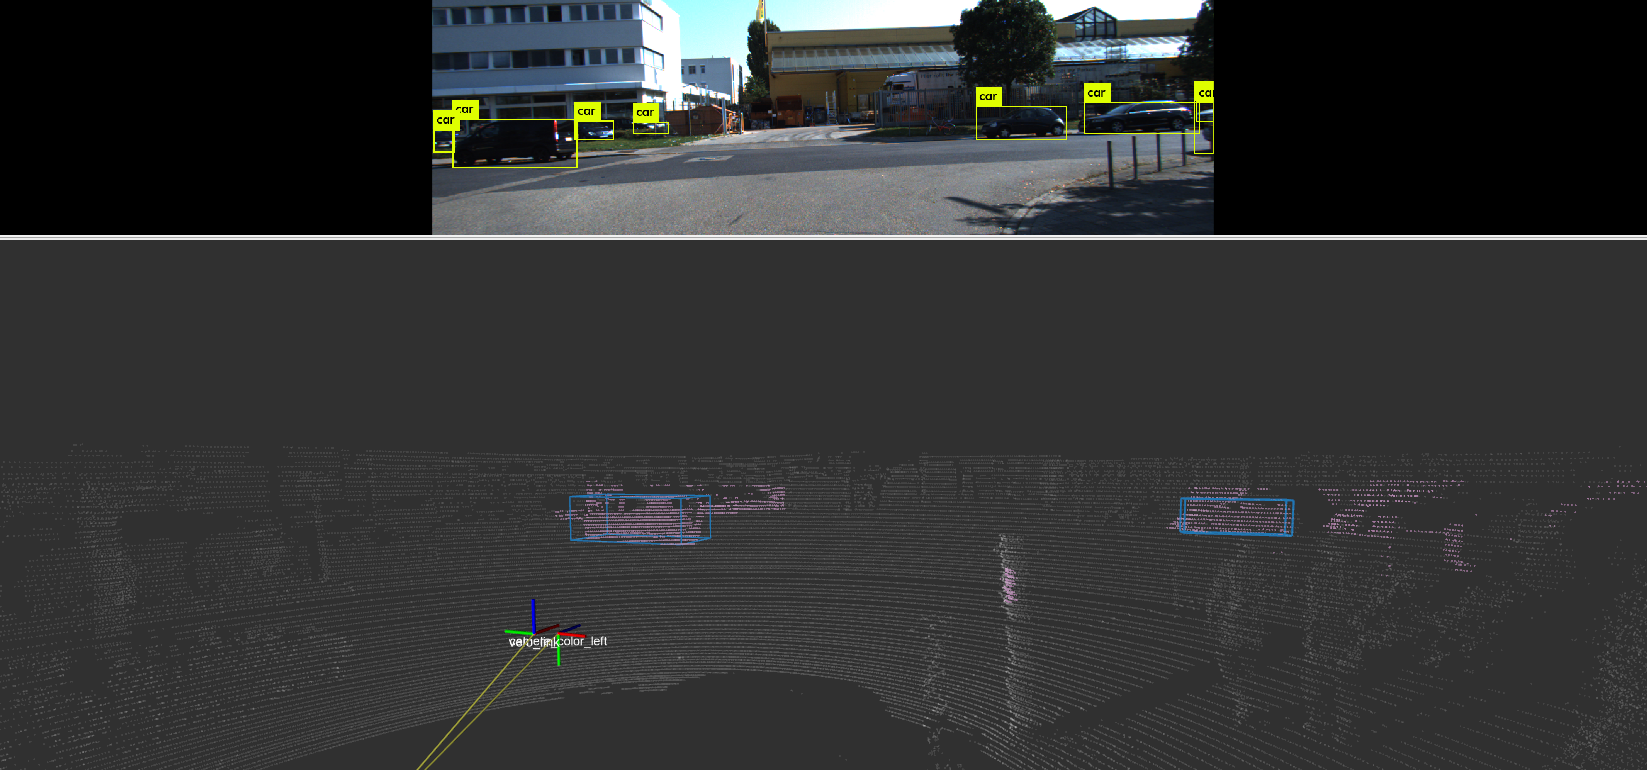
\includegraphics[width=\textwidth]{img/image-object-to-point-cloud/bboxes-side-view.png}
		\caption{In blue, two bounding boxes represented for the two closest cars, of all the \acp{roi} that were projected on the point cloud.}
		\label{fig:bboxes-3d-kitti-side}
	\end{subfigure}
	\caption{Point Cloud tridimensional bounding boxes estimation using the methods described on Sub-section~\ref{subsec:object-detection:bounding-boxes-and-roi}. The 3D bounding boxes are estimated from the image bounding boxes (top of sub-figure). The dark gray point cloud represents the original point cloud gathered by the \ac{lidar} and the lilac zones correspond to the filtered point cloud using \texttt{correspondences\_finder\_node}, node used to filter the original point cloud. In blue, the point cloud bounding boxes are shown, which are estimated from the image bounding boxes, given on the top of the sub-figures. Three different scenarios are presented: side~\subref{fig:bboxes-3d-kitti-side}, front~\subref{fig:bboxes-3d-kitti-front} and top~\subref{fig:bboxes-3d-kitti-top}. The original point cloud is presented using points 4 pixels wide and 10\% of transparency. The filtered point cloud is presented with points 6 pixels wide and 70\% of transparency. Bounding boxes line width is set to \SI{0.1}{\meter}.} 
	\label{fig:bboxes-3d-kitti}
\end{figure}
% Continue the previous figure
\begin{figure}[!ht]\ContinuedFloat
	\centering	
	\begin{subfigure}[c]{0.8\textwidth}
		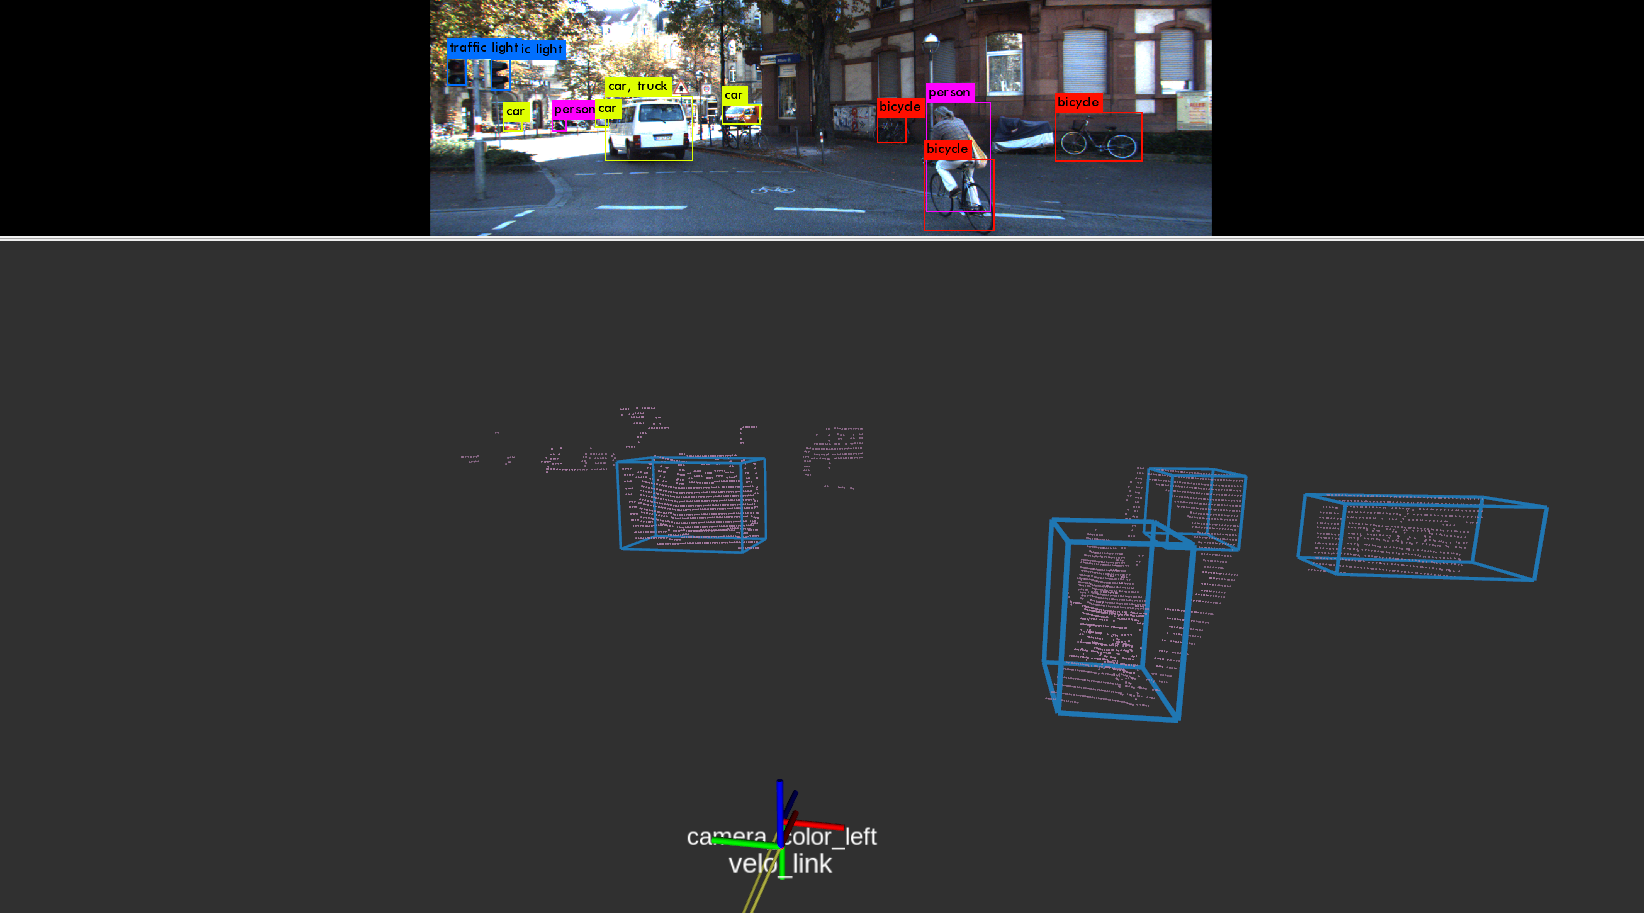
\includegraphics[width=\textwidth]{img/image-object-to-point-cloud/bboxes-front-view.png}
		\caption{On this sub-figure One can notice that not all the point cloud \acp{roi}' are within the bounding box.}
		\label{fig:bboxes-3d-kitti-front}
	\end{subfigure}
	\\ \vspace{4mm}
	\begin{subfigure}[c]{0.8\textwidth}
		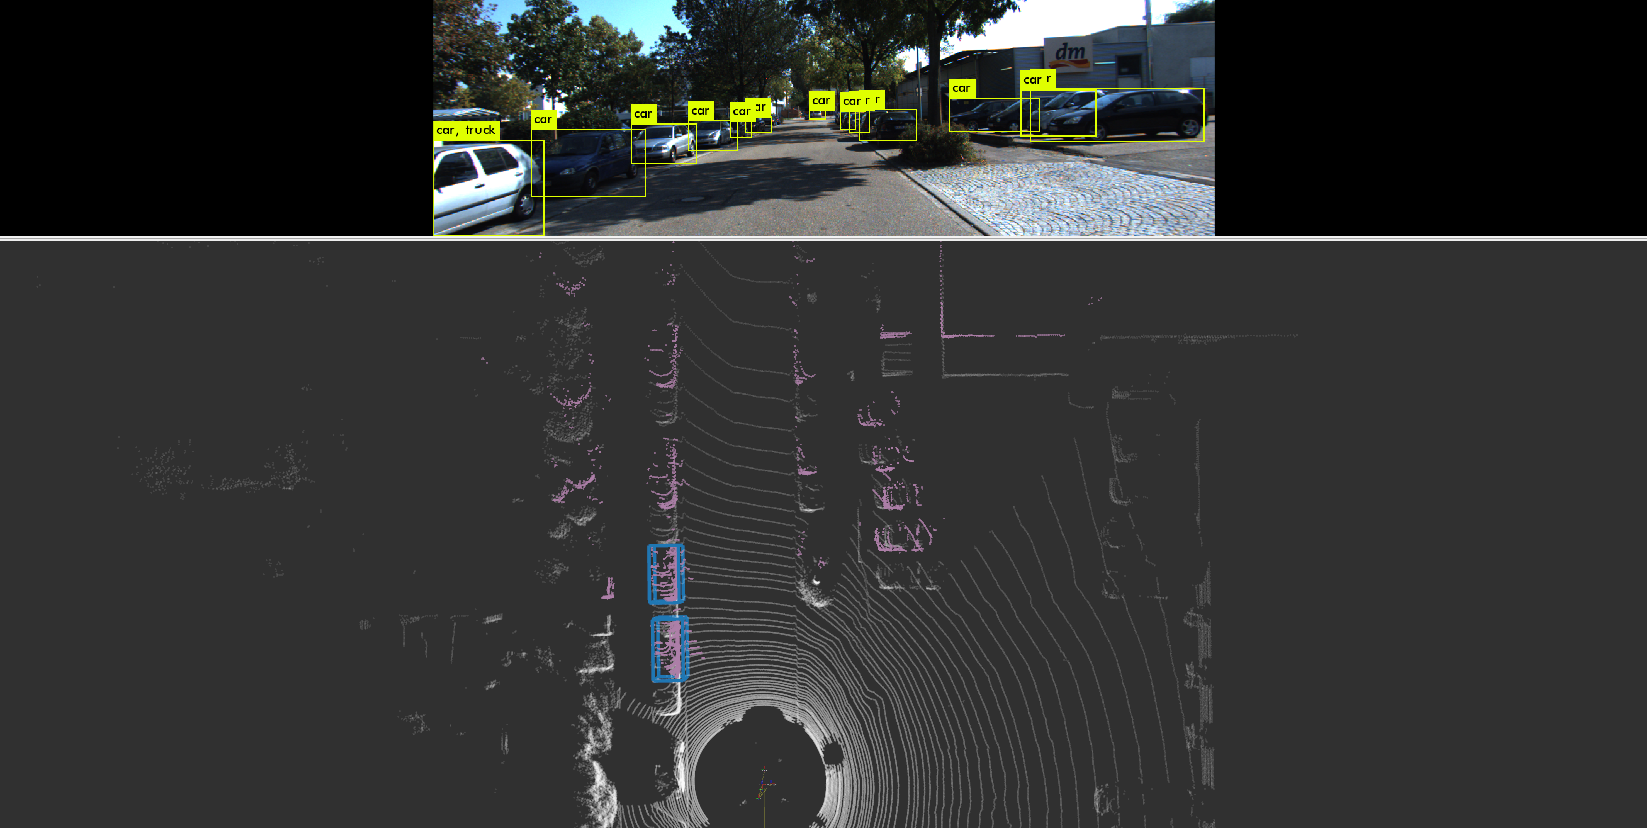
\includegraphics[width=\textwidth]{img/image-object-to-point-cloud/bboxes-top-view.png}
		\caption{Two bounding boxes are presented in blue for the two closest cars, of all the \acp{roi} that were projected on the point cloud. The outliers of the \acp{roi} can also be seen, as several zones of the point cloud are filtered by the \texttt{correspondences\_finder\_node}.}
		\label{fig:bboxes-3d-kitti-top}
	\end{subfigure}
	\caption{Point Cloud tridimensional bounding boxes estimation using the methods described on Sub-section~\ref{subsec:object-detection:bounding-boxes-and-roi}. The 3D bounding boxes are estimated from the image bounding boxes (top of sub-figure). The dark gray point cloud represents the original point cloud gathered by the \ac{lidar} and the lilac zones correspond to the filtered point cloud using \texttt{correspondences\_finder\_node}, node used to filter the original point cloud. In blue, the point cloud bounding boxes are shown, which are estimated from the image bounding boxes, given on the top of the sub-figures. Three different scenarios are presented: side~\subref{fig:bboxes-3d-kitti-side}, front~\subref{fig:bboxes-3d-kitti-front} and top~\subref{fig:bboxes-3d-kitti-top}. The original point cloud is presented using points 4 pixels wide and 10\% of transparency. The filtered point cloud is presented with points 6 pixels wide and 70\% of transparency. Bounding boxes line width is set to \SI{0.1}{\meter}.} 
	\label{fig:bboxes-3d-kitti}
\end{figure}


Despite the promising results, a caveat that is hard to notice is present on the implementation carried. The bounding boxes are of \acl{aabb} type, implying that they are oriented alongside the viewer coordinate frame. On our implementation, this frame is the \texttt{velo\_link}, the \ac{lidar} coordinate frame. Because the \ac{lidar} coordinate frame is not a fixed coordinate frame on the \ac{kitti} dataset, there are some situations where the requirement that the bounding boxes are aligned with the \ac{lidar} coordinate frame axis will force the bounding box to not be aligned with the road direction, specially when the \ac{kitti}'s car does a curve. Such behaviour will still result on a valid bounding box that encloses all the cluster, but its orientation will not coincide with the human perception of the ``correct'' object's bounding box. No attempts of solving this problem were carried. 

\section{Final Remarks}
On this chapter, image object detection is used to identify and crop \aclp{roi} on the point cloud. \ac{yolo} is the \acl{sota} \acl{cnn} selected to perform image object detection, which is integrated with the \ac{ros} network using \texttt{Darknet-ros} package. To determine the equivalent \ac{roi} on the point cloud from the image, two algorithms are developed. The first, establishes $2D \rightarrow 3D$ (from pixels to rays) correspondences and performs frustum filtering on the point cloud; and the second projects tridimensional point cloud points to the image plane, i.e., $3D \rightarrow 2D$ correspondences, selecting the points whose projection is contained on an image bounding box. Considering the accuracy of the \acp{roi} correspondences between image and point cloud, the latter algorithm is preferred, since errors were likely made during the implementation of the former; and the filtered point cloud is voxel filtered and clustered, using \ac{pcl}'s Voxel Grid and Euclidean Cluster filters. 

Such processing chain allows the identification of point cloud clusters that correspond to objects of interest, previously classified by the image object detection. This clusters can then be used for point cloud bounding box estimation and \ac{lidar} interference analysis on objects of interest. Regarding the bounding box estimation, two types are researched: \acf{obb} and \acf{aabb}. Since the goal of bounding box drawing is to show the viewer the objects of interest and their limits, \ac{aabb} are preferred and more intuitive. To speed up the \ac{pcl}'s native implementation of \ac{aabb} computation, the \ac{aabb} position, orientation and dimensions are computed using an alternative method implemented by us, based on \texttt{pcl::getMinMax3D} and high school Euclidean geometry, which yield the similar results and require less than 5\% of the previous execution time.

From this chapter, the main outcome is a processing chain that is capable of extracting the point cloud subsets, representing objects of interest, previously detected on image using image object detection. Such processing chain is relevant to the topic of \ac{lidar} interference since it allows us to analyze the \ac{lidar} interference on objects that are relevant for self-driving vehicles, such as cars, cyclist and pedestrians. The requirements of such implementation are that the camera's and \ac{lidar}'s must be intrinsic calibrated and that their extrinsic calibration must be known.

